\documentclass[12pt,a4paper]{report}

% Packages
\usepackage[utf8]{inputenc}
\usepackage[T1]{fontenc}
\usepackage{geometry}
\usepackage{graphicx}
\usepackage{amsmath}
\usepackage{amssymb}
\usepackage{fancyhdr}
\usepackage{titlesec}
\usepackage{tocloft}
\usepackage{hyperref}
\usepackage{listings}
\usepackage{xcolor}
\usepackage{tikz}
\usetikzlibrary{arrows, positioning, shapes, fit}
\usepackage{float}
\usepackage{caption}
\usepackage{subcaption}
\usepackage{enumitem}
\usepackage{longtable}
\usepackage{booktabs}
\usepackage{array}
\usepackage{multirow}
\usepackage{pdflscape}
\usepackage{afterpage}

% Page setup
\geometry{a4paper, margin=1in}
\setlength{\headheight}{15pt}

% Hyperref setup
\hypersetup{
    colorlinks=true,
    linkcolor=blue,
    filecolor=magenta,      
    urlcolor=cyan,
    pdftitle={Campus-Sync Comprehensive Report},
    pdfauthor={Mausam Kar},
    pdfsubject={Educational Management Platform Report},
    pdfcreator={LaTeX}
}

% Header and footer
\pagestyle{fancy}
\fancyhf{}
\fancyhead[L]{Campus-Sync Report}
\fancyhead[R]{B.Tech Project Exhibition 2024-2025}
\fancyfoot[C]{\leftmark}

% Adjust list spacing
\setlength{\cftbeforetoctitleskip}{0pt}
\setlength{\cftaftertoctitleskip}{0pt}
\setlength{\cftbeforeloftitleskip}{0pt}
\setlength{\cftafterloftitleskip}{0pt}
\setlength{\cftbeforelottitleskip}{0pt}
\setlength{\cftafterlottitleskip}{0pt}

% Reduce spacing in lists of figures and tables
\setlength{\cftfigindent}{0pt}
\setlength{\cftfignumwidth}{3em}
\setlength{\cfttabindent}{0pt}
\setlength{\cfttabnumwidth}{3em}

% Reduce spacing in itemize environments
\setlist[itemize]{topsep=0pt, partopsep=0pt, parsep=0pt, itemsep=0pt}
\setlist[enumerate]{topsep=0pt, partopsep=0pt, parsep=0pt, itemsep=0pt}

% Title format
\titleformat{\chapter}[hang]{\normalfont\Huge\bfseries}{\thechapter}{2pc}{}
\titlespacing*{\chapter}{0pt}{0pt}{20pt}

% Code listing style
\definecolor{codegreen}{rgb}{0,0.6,0}
\definecolor{codegray}{rgb}{0.5,0.5,0.5}
\definecolor{codepurple}{rgb}{0.58,0,0.82}
\definecolor{backcolour}{rgb}{0.95,0.95,0.92}

\lstdefinestyle{mystyle}{
    backgroundcolor=\color{backcolour},
    commentstyle=\color{codegreen},
    keywordstyle=\color{magenta},
    numberstyle=\tiny\color{codegray},
    stringstyle=\color{codepurple},
    basicstyle=\ttfamily\footnotesize,
    breakatwhitespace=false,
    breaklines=true,
    captionpos=b,
    keepspaces=true,
    numbers=left,
    numbersep=5pt,
    showspaces=false,
    showstringspaces=false,
    showtabs=false,
    tabsize=2
}

\lstset{style=mystyle}

% Title
\title{\Huge \textbf{Campus-Sync} \\ \Large Comprehensive Educational Management Platform Report}
\author{Mausam Kar}

\begin{document}

% Custom title page
\begin{titlepage}
    \centering
    \vspace{2cm}
    
    {\LARGE \textbf{Project Report for B.Tech Fall Semester 2024-2025}}\\
    
    \vspace{3cm}
    
    {\Large \textbf{Submitted By:}}\\
    
    \vspace{0.5cm}
    
    {\large
    Mausam Kar (24BAI10248)\\
    Poorna Gupta (24BAI10091)\\
    Krishna Narayan Singh (24BAI10230)\\
    Md Tanzeel Khan (24BAI10359)\\
    Raj Kumar Mahto (24BAI10167)\\
    Nalawde Ashlesh Kumar (24BAI10407)\\
    }
    
    \vspace{2cm}
    
    {\Large \textbf{Under the guidance of}}\\
    
    \vspace{0.5cm}
    
    {\large
    Dr. Trapti Sharma\\
    }
    
    \vspace{3cm}
    
    {\LARGE \textbf{Campus-Sync}}\\
    
    \vspace{0.5cm}
    
    {\Large Comprehensive Educational Management Platform Report}\\
    
    \vspace{2cm}
    
    {\large \today}
    
\end{titlepage}

\thispagestyle{empty}

% Table of contents
\newpage
\tableofcontents
\thispagestyle{empty}

% List of figures
\newpage
\listoffigures
\thispagestyle{empty}

% Chapters
\newpage
\setcounter{page}{1}

\chapter{Introduction}

\section{Project Overview}

Campus-Sync is a modern, comprehensive educational management platform designed to streamline academic operations for students, teachers, and administrators. Built with cutting-edge technologies, it provides a unified solution for managing all aspects of campus life, from academic tracking to wellness features.

The platform addresses the challenges of traditional educational management systems by offering a centralized, role-based interface that enhances productivity, improves communication, and facilitates better academic outcomes. With real-time updates, AI-powered assistance, and a responsive design, Campus-Sync represents the next generation of educational technology solutions.

\section{Project Objectives}

The primary objectives of Campus-Sync include:

\begin{enumerate}[label=\textbf{\arabic*.}]
    \item \textbf{Centralized Management}: Provide a single platform for managing academic, financial, and communication activities.
    \item \textbf{Role-Based Access}: Implement secure, personalized experiences for students, teachers, and administrators.
    \item \textbf{Enhanced Productivity}: Integrate tools like AI assistant, calculators, and wellness features to boost productivity.
    \item \textbf{Real-Time Updates}: Ensure all stakeholders have access to the most current information.
    \item \textbf{Scalability}: Design a modular architecture that can accommodate future growth and feature additions.
\end{enumerate}

\section{Target Users}

Campus-Sync is designed for three primary user groups:

\begin{enumerate}[label=\textbf{\arabic*.}]
    \item \textbf{Students}: Users who need access to academic resources, assignment tracking, grade monitoring, and personal productivity tools.
    \item \textbf{Teachers}: Educators who require tools for class management, assignment creation, grade management, and student analytics.
    \item \textbf{Administrators}: Staff responsible for managing the overall educational environment, including student/teacher management, course planning, and billing systems.
\end{enumerate}

\section{Key Features}

The platform offers a wide range of features organized by user role:

\subsection{Student Features}
\begin{itemize}
    \item Academic Dashboard
    \item Smart Timetable
    \item Assignment Management
    \item Grade Tracking
    \item Expense Tracking
    \item Study Tools
    \item Wellness Features (Meditation, Music, Fitness)
    \item Community Tools
\end{itemize}

\subsection{Teacher Features}
\begin{itemize}
    \item Teaching Dashboard
    \item Class Management
    \item Assignment Creation
    \item Grade Management
    \item Billing System
    \item Exam Management
    \item Student Analytics
\end{itemize}

\subsection{Administrator Features}
\begin{itemize}
    \item Admin Dashboard
    \item Student/Teacher Management
    \item Course Planning
    \item Billing System
    \item Exam Scheduling
    \item Announcement System
    \item Academic Structure Management
\end{itemize}

\subsection{Universal Features}
\begin{itemize}
    \item Role-Based Access Control
    \item Responsive Design
    \item Dark/Light Mode
    \item SEO Optimization
    \item Real-time Updates
    \item AI Assistant
    \item Multimedia Support
    \item Advanced Calculators
\end{itemize}

\section{Technology Stack}

Campus-Sync leverages modern technologies to deliver a robust and scalable solution:

\subsection{Frontend}
\begin{itemize}
    \item React 18
    \item TypeScript
    \item Vite
    \item Tailwind CSS
    \item shadcn/ui
    \item React Router v6
    \item React Hook Form + Zod
    \item Recharts
    \item Lucide React
\end{itemize}

\subsection{Backend \& Services}
\begin{itemize}
    \item Supabase (PostgreSQL, Authentication, Real-time, Edge Functions)
    \item AI Assistant (custom integration)
\end{itemize}

\subsection{Development Tools}
\begin{itemize}
    \item ESLint
    \item PostCSS
    \item TypeScript
    \item Vite
\end{itemize}

This report provides a comprehensive overview of the Campus-Sync platform, detailing its architecture, implementation, features, and future development plans.
\chapter{System Architecture}

\section{Architecture Overview}

Campus-Sync follows a modern, scalable architecture designed to support a panel-based educational management platform. The system is built using a client-server model with a React frontend and Supabase backend, providing a seamless user experience across all roles.

The architecture is organized around three primary user panels (Student, Teacher, and Admin) with shared services that facilitate communication and data exchange between these panels. This design ensures that each user type has access to role-specific features while maintaining a consistent and integrated platform experience.

\section{High-Level Architecture}

\begin{figure}[H]
    \centering
    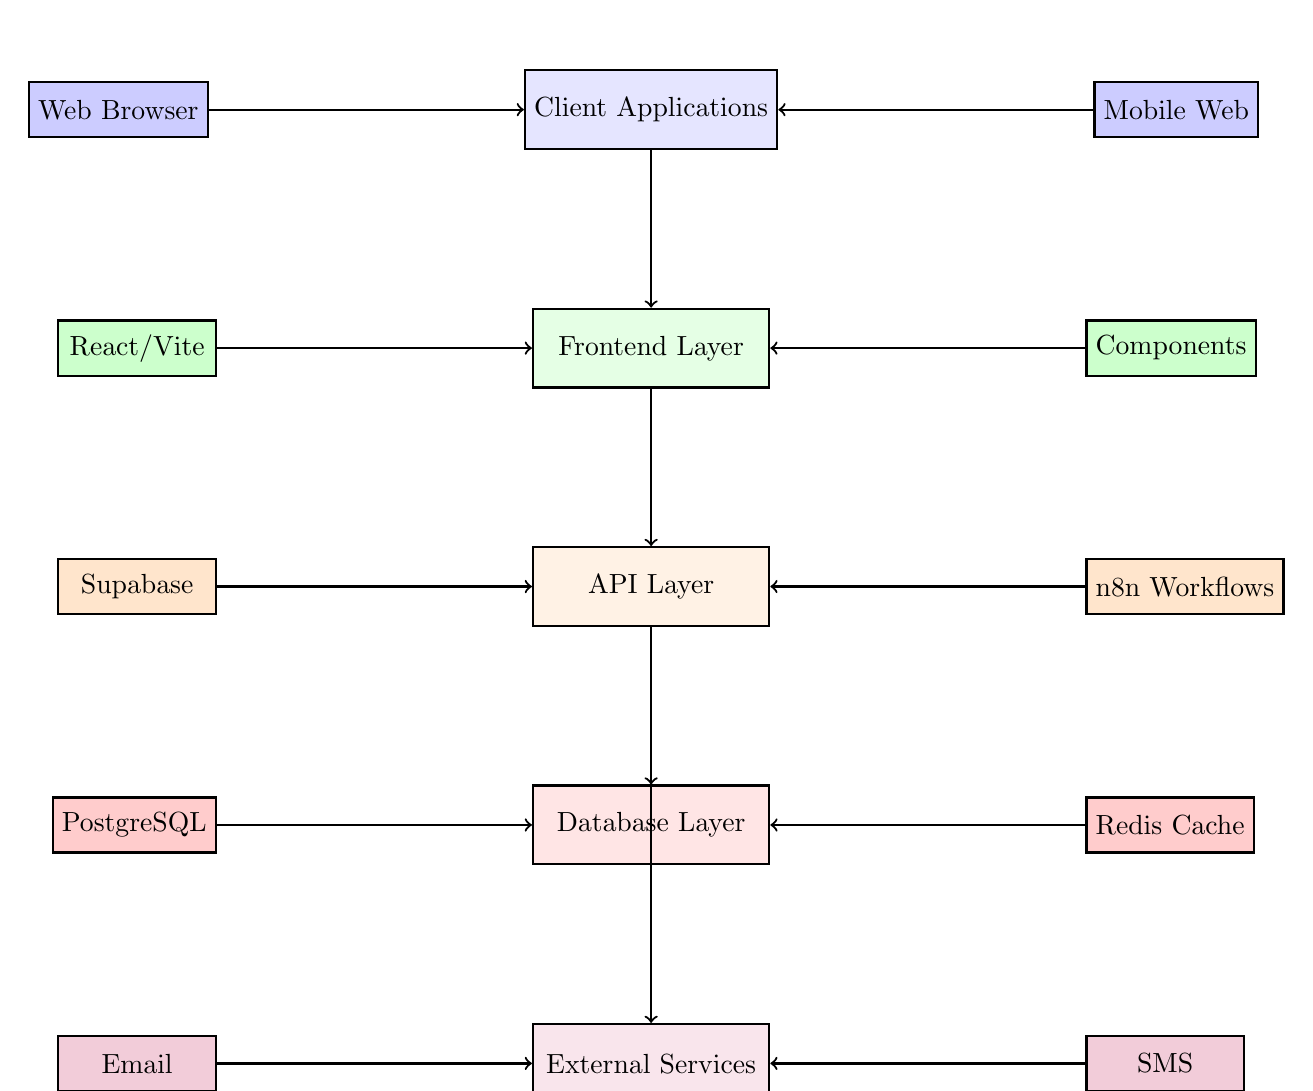
\begin{tikzpicture}[thick, node distance=2cm]
        % Client Applications
        \node (client) [draw, rectangle, minimum width=3cm, minimum height=1cm, fill=blue!10] {Client Applications};
        
        % Frontend Layer
        \node (frontend) [draw, rectangle, minimum width=3cm, minimum height=1cm, fill=green!10, below=of client] {Frontend Layer};
        
        % API Layer
        \node (api) [draw, rectangle, minimum width=3cm, minimum height=1cm, fill=orange!10, below=of frontend] {API Layer};
        
        % Database Layer
        \node (database) [draw, rectangle, minimum width=3cm, minimum height=1cm, fill=red!10, below=of api] {Database Layer};
        
        % External Services
        \node (external) [draw, rectangle, minimum width=3cm, minimum height=1cm, fill=purple!10, below=of database] {External Services};
        
        % Arrows
        \draw[->] (client) -- (frontend);
        \draw[->] (frontend) -- (api);
        \draw[->] (api) -- (database);
        \draw[->] (api) -- (external);
        
        % Subcomponents
        \node (web) [draw, rectangle, minimum width=2cm, minimum height=0.7cm, fill=blue!20, left=of client, xshift=-2cm] {Web Browser};
        \node (mobile) [draw, rectangle, minimum width=2cm, minimum height=0.7cm, fill=blue!20, right=of client, xshift=2cm] {Mobile Web};
        
        \node (react) [draw, rectangle, minimum width=2cm, minimum height=0.7cm, fill=green!20, left=of frontend, xshift=-2cm] {React/Vite};
        \node (components) [draw, rectangle, minimum width=2cm, minimum height=0.7cm, fill=green!20, right=of frontend, xshift=2cm] {Components};
        
        \node (supabase) [draw, rectangle, minimum width=2cm, minimum height=0.7cm, fill=orange!20, left=of api, xshift=-2cm] {Supabase};
        \node (workflows) [draw, rectangle, minimum width=2cm, minimum height=0.7cm, fill=orange!20, right=of api, xshift=2cm] {n8n Workflows};
        
        \node (postgres) [draw, rectangle, minimum width=2cm, minimum height=0.7cm, fill=red!20, left=of database, xshift=-2cm] {PostgreSQL};
        \node (redis) [draw, rectangle, minimum width=2cm, minimum height=0.7cm, fill=red!20, right=of database, xshift=2cm] {Redis Cache};
        
        \node (email) [draw, rectangle, minimum width=2cm, minimum height=0.7cm, fill=purple!20, left=of external, xshift=-2cm] {Email};
        \node (sms) [draw, rectangle, minimum width=2cm, minimum height=0.7cm, fill=purple!20, right=of external, xshift=2cm] {SMS};
        
        % Subcomponent arrows
        \draw[->] (web) -- (client);
        \draw[->] (mobile) -- (client);
        \draw[->] (react) -- (frontend);
        \draw[->] (components) -- (frontend);
        \draw[->] (supabase) -- (api);
        \draw[->] (workflows) -- (api);
        \draw[->] (postgres) -- (database);
        \draw[->] (redis) -- (database);
        \draw[->] (email) -- (external);
        \draw[->] (sms) -- (external);
    \end{tikzpicture}
    \caption{High-Level System Architecture}
    \label{fig:high-level-architecture}
\end{figure}

\section{Panel-Based Architecture}

\begin{figure}[H]
    \centering
    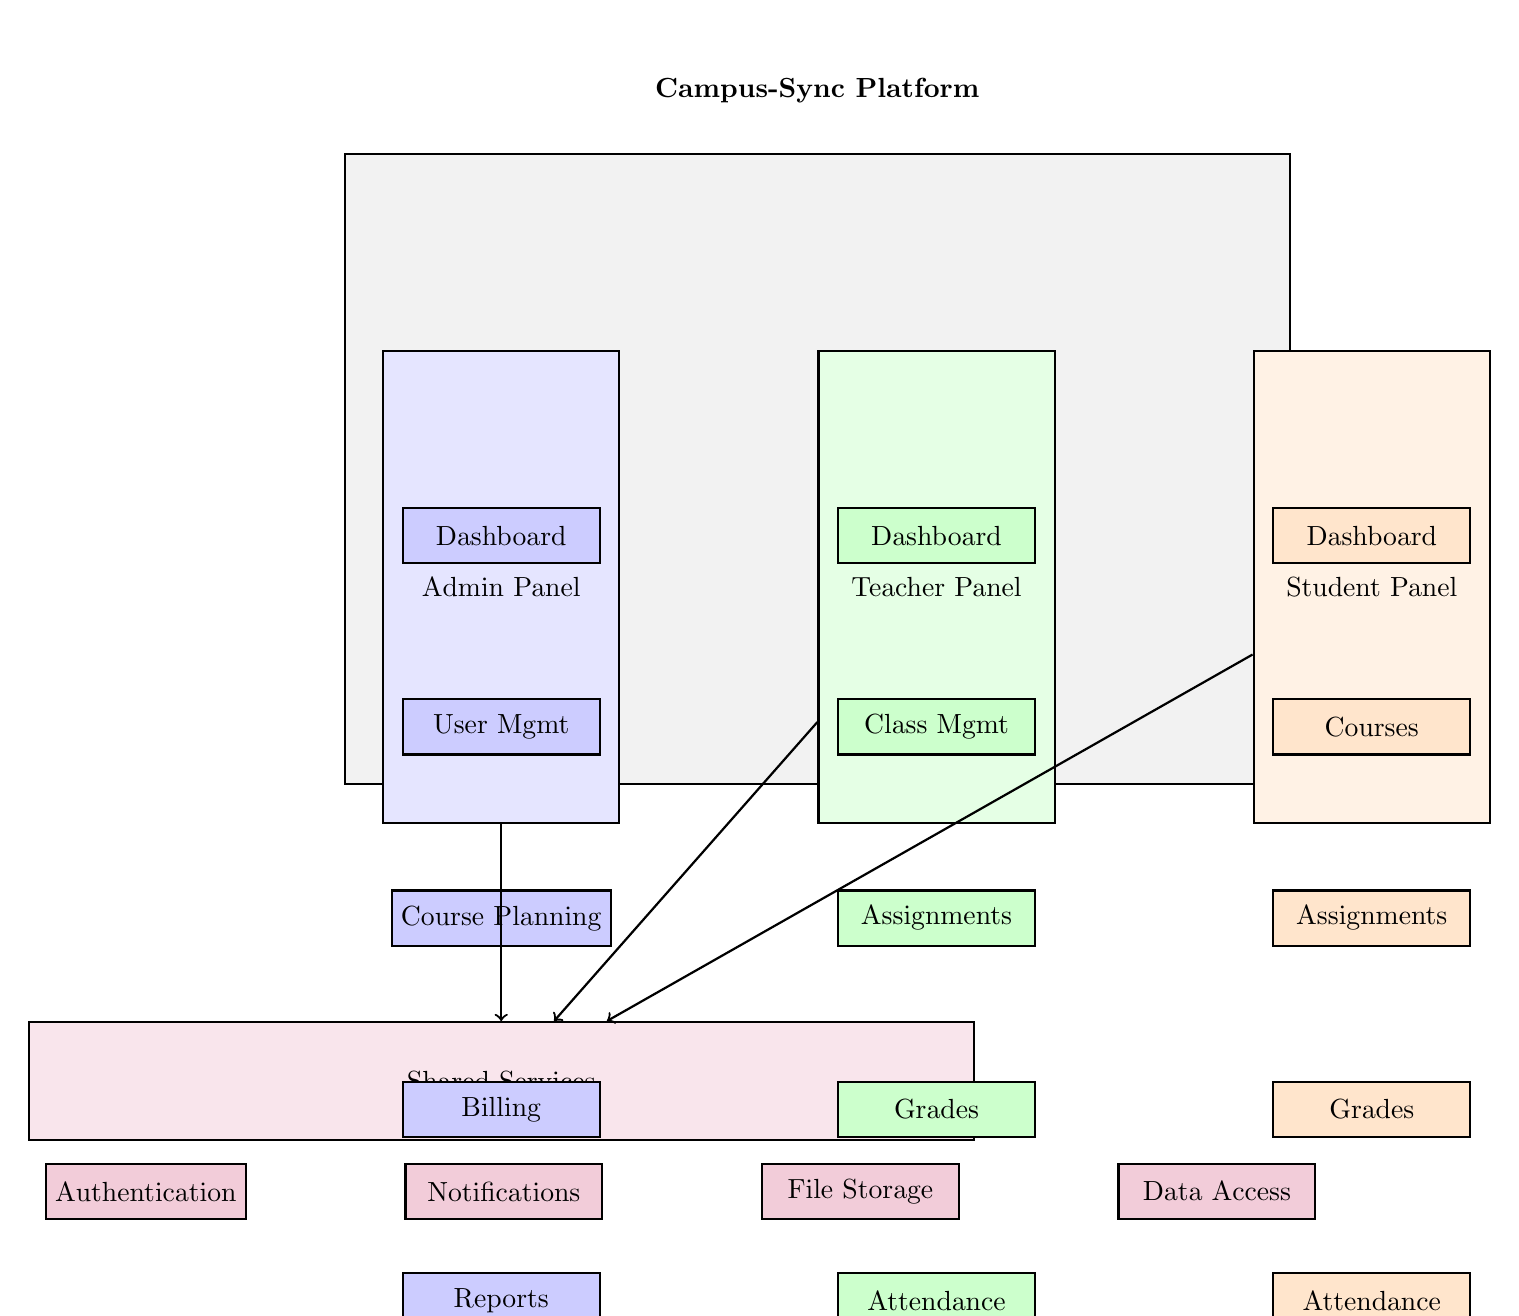
\begin{tikzpicture}[thick, node distance=1.5cm]
        % Main Platform
        \node (platform) [draw, rectangle, minimum width=12cm, minimum height=8cm, fill=gray!10] {};
        \node at (platform.north) [above=0.5cm, font=\bfseries] {Campus-Sync Platform};
        
        % Admin Panel
        \node (admin) [draw, rectangle, minimum width=3cm, minimum height=6cm, fill=blue!10, below=of platform.north west, yshift=-1cm, xshift=2cm] {Admin Panel};
        
        % Teacher Panel
        \node (teacher) [draw, rectangle, minimum width=3cm, minimum height=6cm, fill=green!10, right=of admin, xshift=1cm] {Teacher Panel};
        
        % Student Panel
        \node (student) [draw, rectangle, minimum width=3cm, minimum height=6cm, fill=orange!10, right=of teacher, xshift=1cm] {Student Panel};
        
        % Shared Services
        \node (shared) [draw, rectangle, minimum width=12cm, minimum height=1.5cm, fill=purple!10, below=of admin, yshift=-1cm] {Shared Services};
        
        % Admin Components
        \node (admindash) [draw, rectangle, minimum width=2.5cm, minimum height=0.7cm, fill=blue!20, below=of admin.north, yshift=-0.5cm] {Dashboard};
        \node (usermgmt) [draw, rectangle, minimum width=2.5cm, minimum height=0.7cm, fill=blue!20, below=of admindash, yshift=-0.2cm] {User Mgmt};
        \node (courseplan) [draw, rectangle, minimum width=2.5cm, minimum height=0.7cm, fill=blue!20, below=of usermgmt, yshift=-0.2cm] {Course Planning};
        \node (billing) [draw, rectangle, minimum width=2.5cm, minimum height=0.7cm, fill=blue!20, below=of courseplan, yshift=-0.2cm] {Billing};
        \node (reports) [draw, rectangle, minimum width=2.5cm, minimum height=0.7cm, fill=blue!20, below=of billing, yshift=-0.2cm] {Reports};
        
        % Teacher Components
        \node (teacherdash) [draw, rectangle, minimum width=2.5cm, minimum height=0.7cm, fill=green!20, below=of teacher.north, yshift=-0.5cm] {Dashboard};
        \node (classmgmt) [draw, rectangle, minimum width=2.5cm, minimum height=0.7cm, fill=green!20, below=of teacherdash, yshift=-0.2cm] {Class Mgmt};
        \node (assignments) [draw, rectangle, minimum width=2.5cm, minimum height=0.7cm, fill=green!20, below=of classmgmt, yshift=-0.2cm] {Assignments};
        \node (grades) [draw, rectangle, minimum width=2.5cm, minimum height=0.7cm, fill=green!20, below=of assignments, yshift=-0.2cm] {Grades};
        \node (attendance) [draw, rectangle, minimum width=2.5cm, minimum height=0.7cm, fill=green!20, below=of grades, yshift=-0.2cm] {Attendance};
        
        % Student Components
        \node (studentdash) [draw, rectangle, minimum width=2.5cm, minimum height=0.7cm, fill=orange!20, below=of student.north, yshift=-0.5cm] {Dashboard};
        \node (courses) [draw, rectangle, minimum width=2.5cm, minimum height=0.7cm, fill=orange!20, below=of studentdash, yshift=-0.2cm] {Courses};
        \node (studentassign) [draw, rectangle, minimum width=2.5cm, minimum height=0.7cm, fill=orange!20, below=of courses, yshift=-0.2cm] {Assignments};
        \node (studentgrades) [draw, rectangle, minimum width=2.5cm, minimum height=0.7cm, fill=orange!20, below=of studentassign, yshift=-0.2cm] {Grades};
        \node (studentattend) [draw, rectangle, minimum width=2.5cm, minimum height=0.7cm, fill=orange!20, below=of studentgrades, yshift=-0.2cm] {Attendance};
        
        % Shared Services Components
        \node (auth) [draw, rectangle, minimum width=2.5cm, minimum height=0.7cm, fill=purple!20, below=of shared.north west, yshift=-0.3cm, xshift=1.5cm] {Authentication};
        \node (notifications) [draw, rectangle, minimum width=2.5cm, minimum height=0.7cm, fill=purple!20, right=of auth, xshift=0.5cm] {Notifications};
        \node (storage) [draw, rectangle, minimum width=2.5cm, minimum height=0.7cm, fill=purple!20, right=of notifications, xshift=0.5cm] {File Storage};
        \node (dataaccess) [draw, rectangle, minimum width=2.5cm, minimum height=0.7cm, fill=purple!20, right=of storage, xshift=0.5cm] {Data Access};
        
        % Arrows
        \draw[->] (admin) -- (shared);
        \draw[->] (teacher) -- (shared);
        \draw[->] (student) -- (shared);
    \end{tikzpicture}
    \caption{Panel-Based System Architecture}
    \label{fig:panel-architecture}
\end{figure}

\section{Frontend Architecture}

\begin{figure}[H]
    \centering
    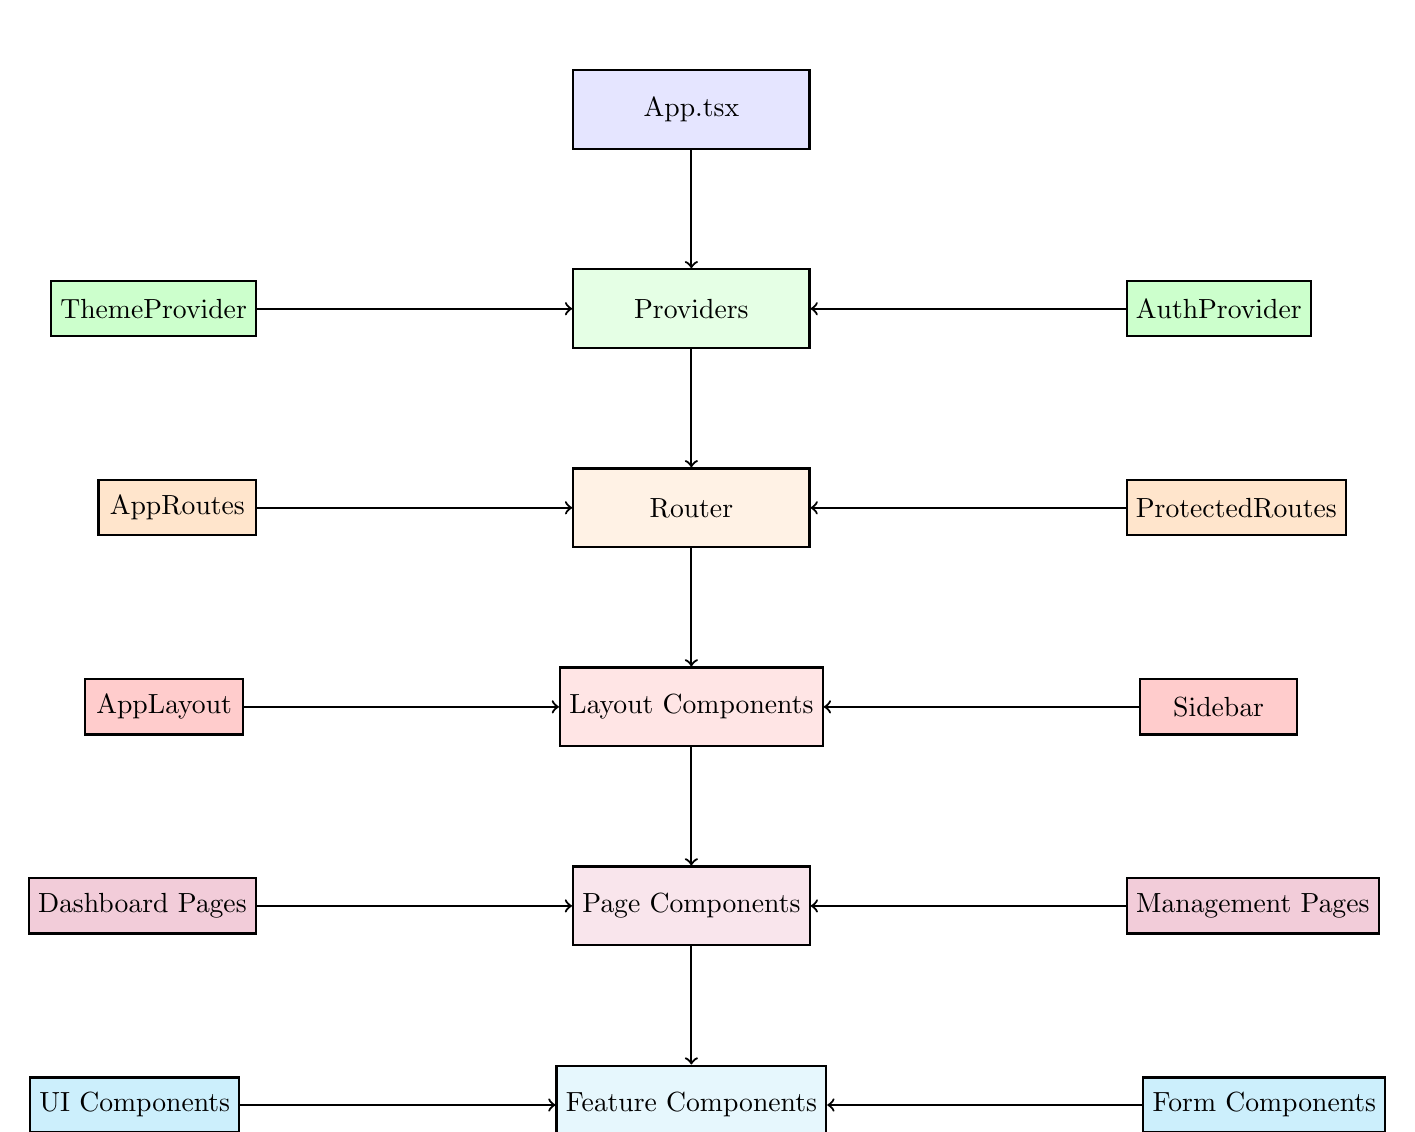
\begin{tikzpicture}[thick, node distance=1.5cm]
        % App Component
        \node (app) [draw, rectangle, minimum width=3cm, minimum height=1cm, fill=blue!10] {App.tsx};
        
        % Providers
        \node (providers) [draw, rectangle, minimum width=3cm, minimum height=1cm, fill=green!10, below=of app] {Providers};
        
        % Router
        \node (router) [draw, rectangle, minimum width=3cm, minimum height=1cm, fill=orange!10, below=of providers] {Router};
        
        % Layout Components
        \node (layout) [draw, rectangle, minimum width=3cm, minimum height=1cm, fill=red!10, below=of router] {Layout Components};
        
        % Page Components
        \node (pages) [draw, rectangle, minimum width=3cm, minimum height=1cm, fill=purple!10, below=of layout] {Page Components};
        
        % Feature Components
        \node (features) [draw, rectangle, minimum width=3cm, minimum height=1cm, fill=cyan!10, below=of pages] {Feature Components};
        
        % Arrows
        \draw[->] (app) -- (providers);
        \draw[->] (providers) -- (router);
        \draw[->] (router) -- (layout);
        \draw[->] (layout) -- (pages);
        \draw[->] (pages) -- (features);
        
        % Subcomponents
        \node (theme) [draw, rectangle, minimum width=2cm, minimum height=0.7cm, fill=green!20, left=of providers, xshift=-2.5cm] {ThemeProvider};
        \node (auth) [draw, rectangle, minimum width=2cm, minimum height=0.7cm, fill=green!20, right=of providers, xshift=2.5cm] {AuthProvider};
        
        \node (approutes) [draw, rectangle, minimum width=2cm, minimum height=0.7cm, fill=orange!20, left=of router, xshift=-2.5cm] {AppRoutes};
        \node (protected) [draw, rectangle, minimum width=2cm, minimum height=0.7cm, fill=orange!20, right=of router, xshift=2.5cm] {ProtectedRoutes};
        
        \node (applayout) [draw, rectangle, minimum width=2cm, minimum height=0.7cm, fill=red!20, left=of layout, xshift=-2.5cm] {AppLayout};
        \node (sidebar) [draw, rectangle, minimum width=2cm, minimum height=0.7cm, fill=red!20, right=of layout, xshift=2.5cm] {Sidebar};
        
        \node (dashpages) [draw, rectangle, minimum width=2cm, minimum height=0.7cm, fill=purple!20, left=of pages, xshift=-2.5cm] {Dashboard Pages};
        \node (mgmtpages) [draw, rectangle, minimum width=2cm, minimum height=0.7cm, fill=purple!20, right=of pages, xshift=2.5cm] {Management Pages};
        
        \node (uicomponents) [draw, rectangle, minimum width=2cm, minimum height=0.7cm, fill=cyan!20, left=of features, xshift=-2.5cm] {UI Components};
        \node (formcomponents) [draw, rectangle, minimum width=2cm, minimum height=0.7cm, fill=cyan!20, right=of features, xshift=2.5cm] {Form Components};
        
        % Subcomponent arrows
        \draw[->] (theme) -- (providers);
        \draw[->] (auth) -- (providers);
        \draw[->] (approutes) -- (router);
        \draw[->] (protected) -- (router);
        \draw[->] (applayout) -- (layout);
        \draw[->] (sidebar) -- (layout);
        \draw[->] (dashpages) -- (pages);
        \draw[->] (mgmtpages) -- (pages);
        \draw[->] (uicomponents) -- (features);
        \draw[->] (formcomponents) -- (features);
    \end{tikzpicture}
    \caption{Frontend Component Hierarchy}
    \label{fig:frontend-hierarchy}
\end{figure}

\section{Backend Architecture}

\begin{figure}[H]
    \centering
    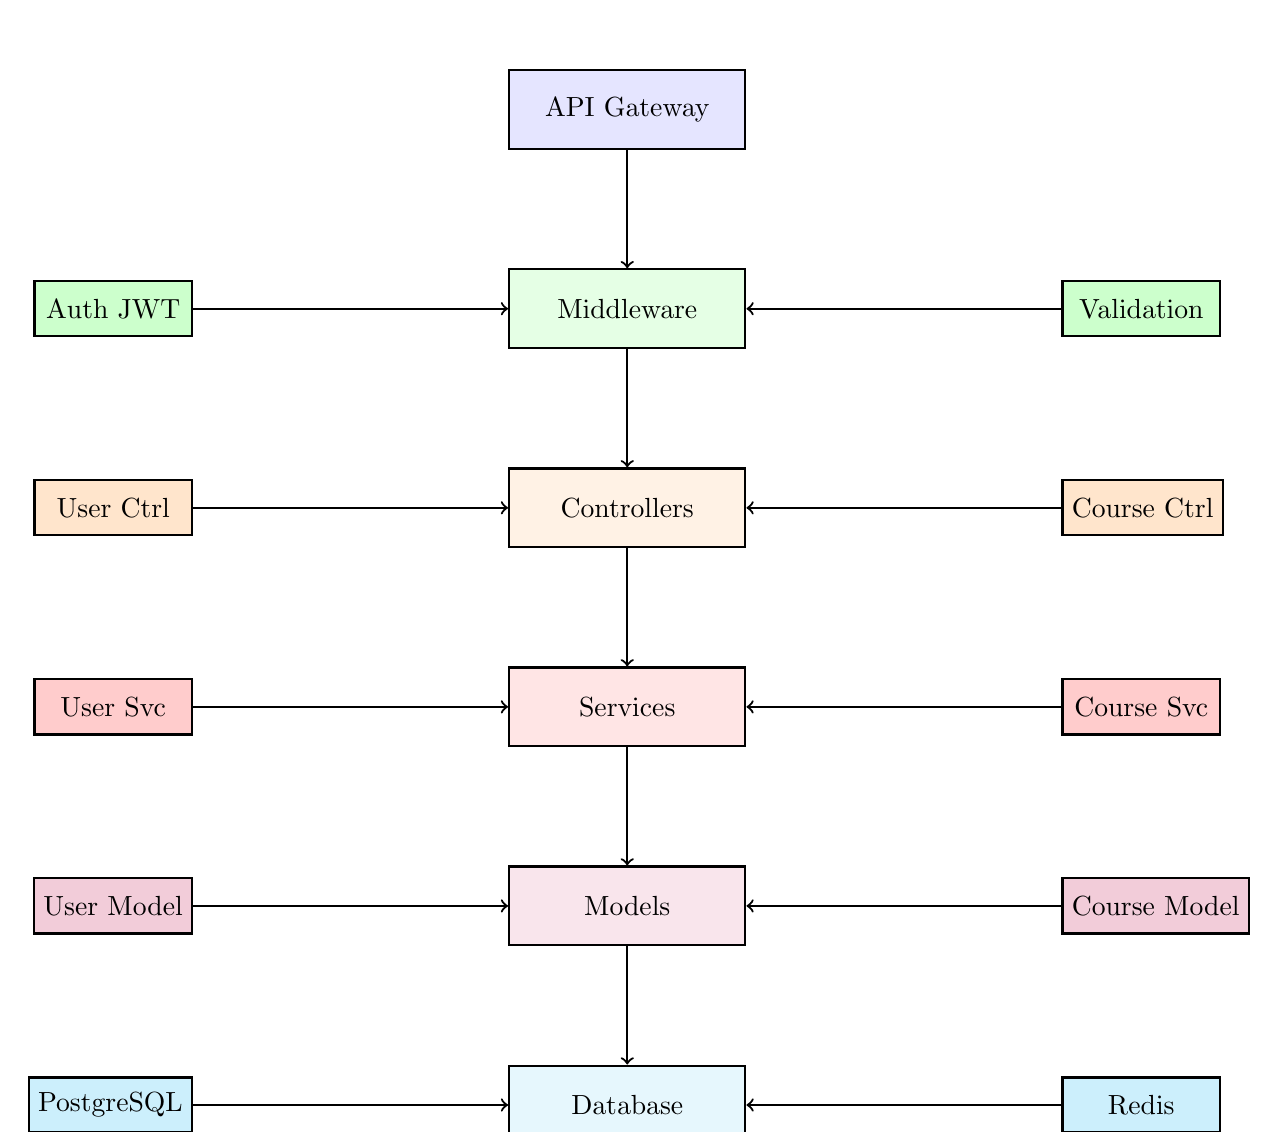
\begin{tikzpicture}[thick, node distance=1.5cm]
        % API Gateway
        \node (api) [draw, rectangle, minimum width=3cm, minimum height=1cm, fill=blue!10] {API Gateway};
        
        % Middleware
        \node (middleware) [draw, rectangle, minimum width=3cm, minimum height=1cm, fill=green!10, below=of api] {Middleware};
        
        % Controllers
        \node (controllers) [draw, rectangle, minimum width=3cm, minimum height=1cm, fill=orange!10, below=of middleware] {Controllers};
        
        % Services
        \node (services) [draw, rectangle, minimum width=3cm, minimum height=1cm, fill=red!10, below=of controllers] {Services};
        
        % Models
        \node (models) [draw, rectangle, minimum width=3cm, minimum height=1cm, fill=purple!10, below=of services] {Models};
        
        % Database
        \node (database) [draw, rectangle, minimum width=3cm, minimum height=1cm, fill=cyan!10, below=of models] {Database};
        
        % Arrows
        \draw[->] (api) -- (middleware);
        \draw[->] (middleware) -- (controllers);
        \draw[->] (controllers) -- (services);
        \draw[->] (services) -- (models);
        \draw[->] (models) -- (database);
        
        % Subcomponents
        \node (authjwt) [draw, rectangle, minimum width=2cm, minimum height=0.7cm, fill=green!20, left=of middleware, xshift=-2.5cm] {Auth JWT};
        \node (validation) [draw, rectangle, minimum width=2cm, minimum height=0.7cm, fill=green!20, right=of middleware, xshift=2.5cm] {Validation};
        
        \node (userctrl) [draw, rectangle, minimum width=2cm, minimum height=0.7cm, fill=orange!20, left=of controllers, xshift=-2.5cm] {User Ctrl};
        \node (coursectrl) [draw, rectangle, minimum width=2cm, minimum height=0.7cm, fill=orange!20, right=of controllers, xshift=2.5cm] {Course Ctrl};
        
        \node (usersvc) [draw, rectangle, minimum width=2cm, minimum height=0.7cm, fill=red!20, left=of services, xshift=-2.5cm] {User Svc};
        \node (coursesvc) [draw, rectangle, minimum width=2cm, minimum height=0.7cm, fill=red!20, right=of services, xshift=2.5cm] {Course Svc};
        
        \node (usermodel) [draw, rectangle, minimum width=2cm, minimum height=0.7cm, fill=purple!20, left=of models, xshift=-2.5cm] {User Model};
        \node (coursemodel) [draw, rectangle, minimum width=2cm, minimum height=0.7cm, fill=purple!20, right=of models, xshift=2.5cm] {Course Model};
        
        \node (postgres) [draw, rectangle, minimum width=2cm, minimum height=0.7cm, fill=cyan!20, left=of database, xshift=-2.5cm] {PostgreSQL};
        \node (redis) [draw, rectangle, minimum width=2cm, minimum height=0.7cm, fill=cyan!20, right=of database, xshift=2.5cm] {Redis};
        
        % Subcomponent arrows
        \draw[->] (authjwt) -- (middleware);
        \draw[->] (validation) -- (middleware);
        \draw[->] (userctrl) -- (controllers);
        \draw[->] (coursectrl) -- (controllers);
        \draw[->] (usersvc) -- (services);
        \draw[->] (coursesvc) -- (services);
        \draw[->] (usermodel) -- (models);
        \draw[->] (coursemodel) -- (models);
        \draw[->] (postgres) -- (database);
        \draw[->] (redis) -- (database);
    \end{tikzpicture}
    \caption{Backend Architecture Layers}
    \label{fig:backend-architecture}
\end{figure}

\section{Data Flow Patterns}

\begin{figure}[H]
    \centering
    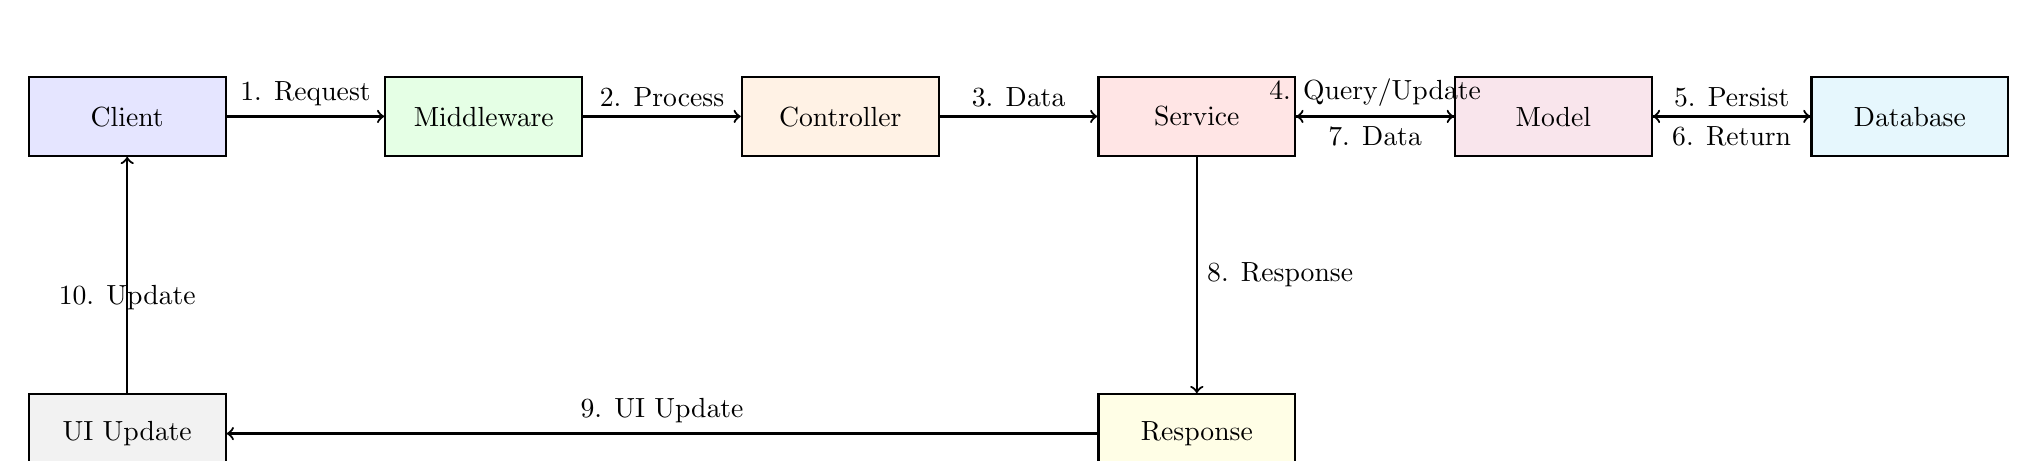
\begin{tikzpicture}[thick, node distance=2cm]
        % Components
        \node (client) [draw, rectangle, minimum width=2.5cm, minimum height=1cm, fill=blue!10] {Client};
        \node (middleware) [draw, rectangle, minimum width=2.5cm, minimum height=1cm, fill=green!10, right=of client] {Middleware};
        \node (controller) [draw, rectangle, minimum width=2.5cm, minimum height=1cm, fill=orange!10, right=of middleware] {Controller};
        \node (service) [draw, rectangle, minimum width=2.5cm, minimum height=1cm, fill=red!10, right=of controller] {Service};
        \node (model) [draw, rectangle, minimum width=2.5cm, minimum height=1cm, fill=purple!10, right=of service] {Model};
        \node (database) [draw, rectangle, minimum width=2.5cm, minimum height=1cm, fill=cyan!10, right=of model] {Database};
        
        % Response path
        \node (response) [draw, rectangle, minimum width=2.5cm, minimum height=1cm, fill=yellow!10, below=of service, yshift=-1cm] {Response};
        \node (ui) [draw, rectangle, minimum width=2.5cm, minimum height=1cm, fill=gray!10, below=of client, yshift=-1cm] {UI Update};
        
        % Arrows
        \draw[->] (client) -- (middleware) node[midway, above] {1. Request};
        \draw[->] (middleware) -- (controller) node[midway, above] {2. Process};
        \draw[->] (controller) -- (service) node[midway, above] {3. Data};
        \draw[->] (service) -- (model) node[midway, above] {4. Query/Update};
        \draw[->] (model) -- (database) node[midway, above] {5. Persist};
        \draw[->] (database) -- (model) node[midway, below] {6. Return};
        \draw[->] (model) -- (service) node[midway, below] {7. Data};
        \draw[->] (service) -- (response) node[midway, right] {8. Response};
        \draw[->] (response) -- (ui) node[midway, above] {9. UI Update};
        \draw[->] (ui) -- (client) node[midway, below] {10. Update};
    \end{tikzpicture}
    \caption{Data Flow Pattern}
    \label{fig:data-flow}
\end{figure}

\section{Security Architecture}

\begin{figure}[H]
    \centering
    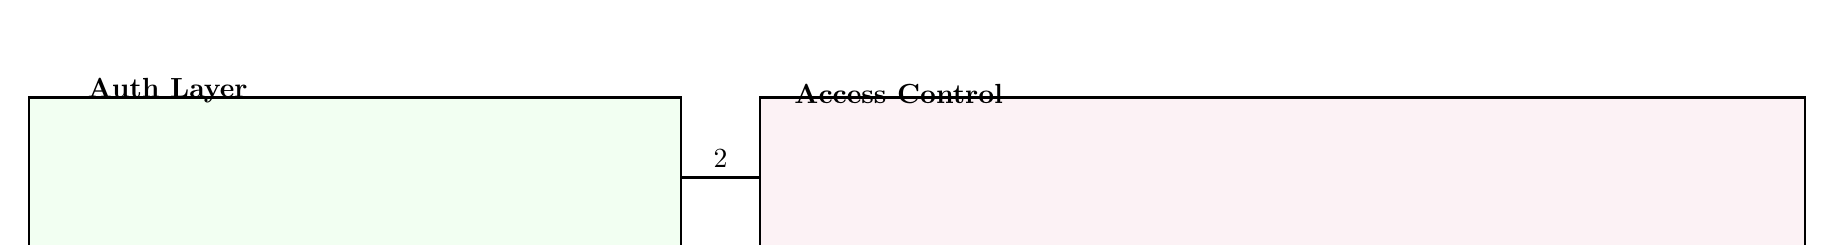
\begin{tikzpicture}[thick, node distance=2cm]
        % Components
        \node (user) [draw, rectangle, minimum width=2.5cm, minimum height=1cm, fill=blue!10] {User Request};
        \node (jwt) [draw, rectangle, minimum width=2.5cm, minimum height=1cm, fill=green!10, right=of user] {JWT Validation};
        \node (role) [draw, rectangle, minimum width=2.5cm, minimum height=1cm, fill=orange!10, right=of jwt] {Role Check};
        \node (permission) [draw, rectangle, minimum width=2.5cm, minimum height=1cm, fill=red!10, right=of role] {Permission Check};
        \node (resource) [draw, rectangle, minimum width=2.5cm, minimum height=1cm, fill=purple!10, right=of permission] {Resource Access};
        
        % Arrows
        \draw[->] (user) -- (jwt) node[midway, above] {1};
        \draw[->] (jwt) -- (role) node[midway, above] {2};
        \draw[->] (role) -- (permission) node[midway, above] {3};
        \draw[->] (permission) -- (resource) node[midway, above] {4};
        
        % Layers
        \node[draw, rectangle, minimum width=6cm, minimum height=2cm, fill=green!5, fit=(user) (jwt), inner sep=0.5cm] {};
        \node at (jwt.north -| user) [above=0.3cm, font=\bfseries] {Auth Layer};
        
        \node[draw, rectangle, minimum width=6cm, minimum height=2cm, fill=purple!5, fit=(role) (resource), inner sep=0.5cm] {};
        \node at (resource.north -| role) [above=0.3cm, font=\bfseries] {Access Control};
    \end{tikzpicture}
    \caption{Security Architecture Flow}
    \label{fig:security-flow}
\end{figure}

This architecture provides a solid foundation for the Campus-Sync platform, ensuring scalability, maintainability, and security across all components.
\chapter{Frontend Implementation}

\section{Technology Stack}

The frontend of Campus-Sync is built using modern web technologies that provide a responsive, performant, and maintainable user interface:

\begin{itemize}
    \item \textbf{React 18}: A JavaScript library for building user interfaces with component-based architecture
    \item \textbf{TypeScript}: A typed superset of JavaScript that compiles to plain JavaScript
    \item \textbf{Vite}: A next-generation frontend tooling that provides fast development and build processes
    \item \textbf{Tailwind CSS}: A utility-first CSS framework for rapidly building custom user interfaces
    \item \textbf{shadcn/ui}: A collection of accessible, customizable UI components built with Radix UI and Tailwind CSS
    \item \textbf{React Router v6}: Declarative routing for React applications
    \item \textbf{React Hook Form}: Performant, flexible forms with easy validation
    \item \textbf{Zod}: TypeScript-first schema declaration and validation library
    \item \textbf{Recharts}: A composable charting library built on React components
    \item \textbf{Lucide React}: A library of simply beautiful open source icons
\end{itemize}

\section{Component Architecture}

The frontend follows a modular component architecture with clear separation of concerns. Components are organized in a hierarchical structure:

\subsection{Component Hierarchy}

\begin{figure}[H]
    \centering
    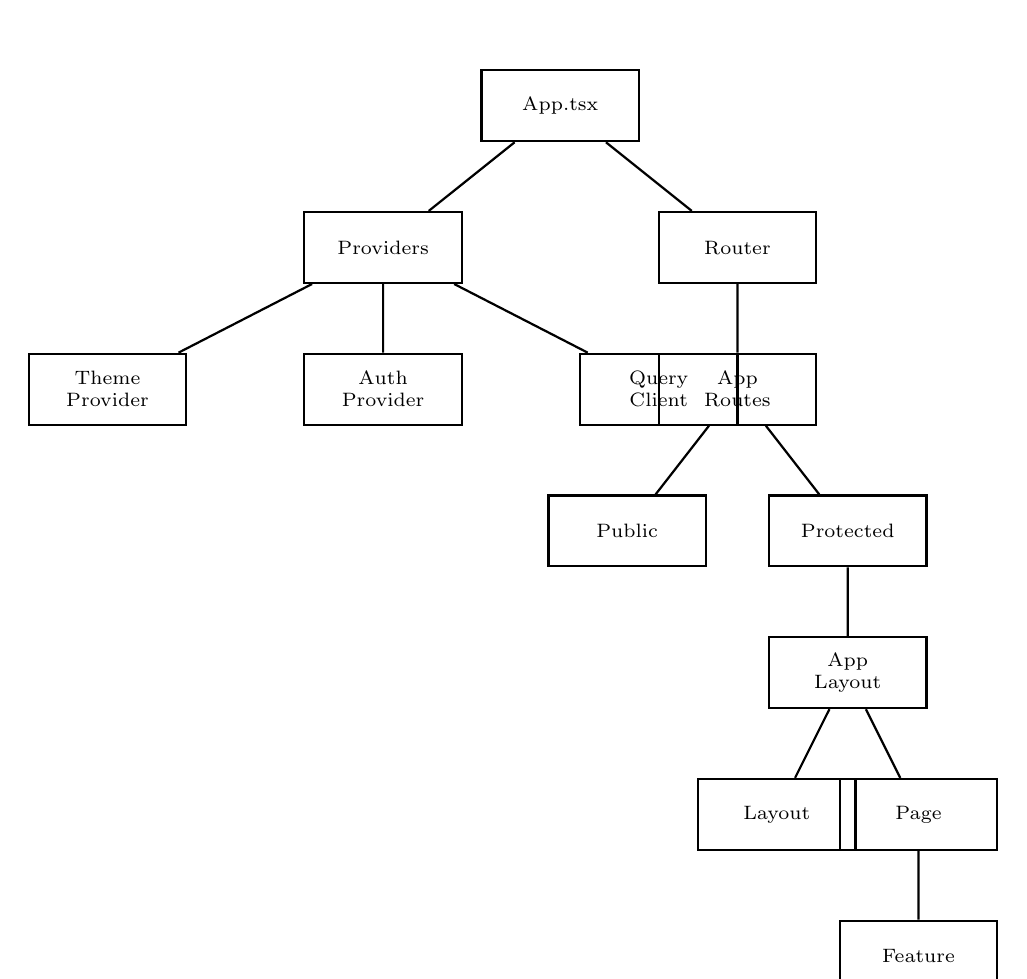
\begin{tikzpicture}[thick, level distance=1.8cm,
      level 1/.style={sibling distance=4.5cm},
      level 2/.style={sibling distance=3.5cm},
      level 3/.style={sibling distance=2.8cm},
      level 4/.style={sibling distance=2.2cm},
      level 5/.style={sibling distance=1.8cm},
      level 6/.style={sibling distance=1.5cm},
      every node/.style={align=center, rectangle, draw, minimum width=2cm, minimum height=0.9cm, font=\scriptsize}]
      \node {App.tsx}
        child { node {Providers}
          child { node {Theme\\Provider} }
          child { node {Auth\\Provider} }
          child { node {Query\\Client} }
        }
        child { node {Router}
          child { node {App\\Routes}
            child { node {Public} }
            child { node {Protected}
              child { node {App\\Layout}
                child { node {Layout} }
                child { node {Page}
                  child { node {Feature} }
                }
              }
            }
          }
        };
    \end{tikzpicture}
    \caption{Component Hierarchy Tree}
    \label{fig:component-hierarchy}
\end{figure}

\subsection{Folder Structure}

The frontend codebase is organized into the following directory structure:

\begin{verbatim}
src/
├── assets/               # Static assets (images, icons, etc.)
├── components/           # Reusable UI components
│   ├── about/            # About page components
│   ├── admin/            # Admin-specific components
│   ├── announcements/    # Announcement components
│   ├── assignments/      # Assignment components
│   ├── attendance/       # Attendance components
│   ├── auth/             # Authentication components
│   ├── billing/          # Billing components
│   ├── calculators/      # Calculator components
│   ├── community/        # Community components
│   ├── courses/          # Course components
│   ├── dashboard/        # Dashboard components
│   ├── exams/            # Exam components
│   ├── expenses/         # Expense components
│   ├── features/         # Feature components
│   ├── fitness/          # Fitness components
│   ├── layout/           # Layout components
│   ├── marks/            # Marks components
│   ├── meditation/       # Meditation components
│   ├── music/            # Music components
│   ├── mycourses/        # My courses components
│   ├── notes/            # Notes components
│   ├── profile/          # Profile components
│   ├── shared/           # Shared components
│   ├── students/         # Student components
│   ├── ui/               # Base UI components (shadcn/ui)
│   ├── ProtectedRoute.tsx # Route protection component
│   ├── PublicRoute.tsx    # Public route component
│   ├── RoleRoute.tsx      # Role-based route component
│   ├── SEO.tsx           # SEO component
│   ├── ScrollToTop.tsx   # Scroll to top component
│   ├── app-sidebar.tsx   # Application sidebar
│   ├── nav-main.tsx      # Main navigation
│   ├── nav-projects.tsx  # Projects navigation
│   ├── nav-secondary.tsx # Secondary navigation
│   ├── nav-user.tsx      # User navigation
│   ├── theme-provider.tsx # Theme provider
│   └── theme-toggle.tsx  # Theme toggle
├── contexts/             # React context providers
│   └── AuthContext.tsx   # Authentication context
├── data/                 # Static data files
│   └── courseData.ts     # Course data
├── hooks/                # Custom React hooks
│   ├── index.ts          # Hooks exports
│   ├── use-mobile.tsx    # Mobile detection hook
│   ├── use-page-loading.tsx # Page loading hook
│   ├── use-toast.ts      # Toast notification hook
│   ├── useAdminData.ts   # Admin data hook
│   ├── useAdminIDData.ts # Admin ID data hook
│   ├── useAudioPlayer.ts # Audio player hook
│   ├── useLocalStorage.ts # Local storage hook
│   ├── useSEO.ts         # SEO hook
│   ├── useStudentIDData.ts # Student ID data hook
│   ├── useTeacherIDData.ts # Teacher ID data hook
│   └── useUserData.ts    # User data hook
├── lib/                  # Utility libraries
│   ├── index.ts          # Library exports
│   └── utils.ts          # Utility functions
├── pages/                # Page components
│   ├── admin/            # Admin pages
│   ├── student/          # Student pages
│   ├── teacher/          # Teacher pages
│   └── shared/           # Shared pages
├── routes/               # Route definitions
│   ├── admin/            # Admin routes
│   ├── student/          # Student routes
│   ├── teacher/          # Teacher routes
│   ├── common/           # Common routes
│   ├── AppRoutes.tsx     # Main routes
│   ├── ProtectedRoutes.tsx # Protected routes
│   ├── PublicRoutes.tsx  # Public routes
│   └── index.ts          # Routes exports
├── types/                # TypeScript types
│   ├── academic.ts       # Academic types
│   ├── attendance.ts     # Attendance types
│   └── exam.ts           # Exam types
├── App.css               # Global styles
├── App.tsx               # Main application component
├── index.css             # Base styles
├── main.tsx              # Application entry point
└── vite-env.d.ts         # Vite environment types
\end{verbatim}

\section{State Management}

Campus-Sync employs multiple state management strategies depending on the scope and nature of the data:

\subsection{Context API}

The Context API is used for global state management, particularly for authentication and theming:

\begin{itemize}
    \item \textbf{AuthContext}: Manages user authentication state, including login status, user role, and profile information
    \item \textbf{ThemeContext}: Handles dark/light mode preferences and theme-related state
\end{itemize}

\subsection{Custom Hooks}

Custom hooks encapsulate reusable logic and state management patterns:

\begin{itemize}
    \item \textbf{useAuth}: Provides authentication state and methods
    \item \textbf{useUserData}: Manages user-specific data fetching and caching
    \item \textbf{useLocalStorage}: Handles persistent storage in the browser's local storage
    \item \textbf{useMobile}: Detects mobile device usage for responsive design
    \item \textbf{useSEO}: Manages SEO metadata for pages
\end{itemize}

\subsection{React Query}

React Query is used for server state management, providing:

\begin{itemize}
    \item Data caching and synchronization
    \item Background data fetching
    \item Mutation handling
    \item Pagination support
\end{itemize}

\section{Routing Structure}

The application implements a comprehensive routing system with role-based access control:

\subsection{Route Organization}

\begin{itemize}
    \item \textbf{Public Routes}: Authentication pages accessible to all users
    \item \textbf{Protected Routes}: Application features requiring authentication
    \item \textbf{Role Routes}: Panel-specific routes for students, teachers, and administrators
    \item \textbf{Common Routes}: Shared features accessible to all authenticated users
\end{itemize}

\subsection{Navigation Structure}

The navigation system includes:

\begin{itemize}
    \item Main sidebar navigation with role-specific items
    \item Breadcrumb navigation for context awareness
    \item Quick access toolbar for frequently used features
\end{itemize}

\section{UI/UX Design}

The user interface follows modern design principles to ensure an intuitive and engaging user experience.

\subsection{Design System}

\begin{itemize}
    \item \textbf{Color Palette}: Primary, Secondary, Success, Warning, Error, and Neutral colors
    \item \textbf{Typography}: Responsive font sizing with consistent hierarchy
    \item \textbf{Spacing}: 8px base unit with consistent spacing scale
    \item \textbf{Breakpoints}: Mobile (320px), Tablet (768px), Desktop (1024px), Large Desktop (1440px)
\end{itemize}

\subsection{Responsive Design}

\begin{itemize}
    \item Mobile-first approach
    \item Flexible grid system
    \item Touch-friendly interactions
    \item Adaptive layouts for different screen sizes
\end{itemize}

\subsection{Accessibility}

\begin{itemize}
    \item WCAG 2.1 AA compliance
    \item Semantic HTML structure
    \item Keyboard navigation support
    \item Screen reader compatibility
    \item Proper contrast ratios
\end{itemize}

\section{Performance Optimization}

Several optimization techniques are implemented to ensure fast loading and smooth interactions:

\subsection{Code Splitting}

\begin{itemize}
    \item Route-based code splitting
    \item Dynamic imports for heavy components
    \item Lazy loading of non-critical features
\end{itemize}

\subsection{Bundle Optimization}

\begin{itemize}
    \item Tree shaking for unused code
    \item Minification and compression
    \item Image optimization
    \item Font loading optimization
\end{itemize}

\subsection{Caching Strategy}

\begin{itemize}
    \item Browser caching for static assets
    \item Service worker for offline support
    \item React Query caching for API responses
    \item Local storage for user preferences
\end{itemize}

\section{Authentication and Authorization}

The authentication system implements JWT-based security with role-based access control:

\subsection{Authentication Flow}

\begin{enumerate}
    \item User visits authentication page
    \item Credentials submitted to backend
    \item JWT tokens received and stored
    \item User redirected to appropriate dashboard
    \item Tokens refreshed automatically before expiry
\end{enumerate}

\subsection{Role-Based Access Control}

\begin{itemize}
    \item \textbf{Student}: Access to student dashboard, courses, assignments, grades
    \item \textbf{Teacher}: Access to teacher dashboard, class management, grading
    \item \textbf{Admin}: Access to admin dashboard, user management, system settings
\end{itemize}

This frontend implementation provides a solid foundation for the Campus-Sync platform, ensuring a responsive, accessible, and performant user experience across all devices and user roles.
\chapter{Backend Implementation}

\section{Technology Stack}

The backend of Campus-Sync is built using a modern, scalable technology stack designed to handle the complex requirements of an educational management platform:

\begin{itemize}
    \item \textbf{Express.js}: A minimal and flexible Node.js web application framework
    \item \textbf{MongoDB}: A document-based NoSQL database for flexible data storage
    \item \textbf{Mongoose}: An Object Data Modeling (ODM) library for MongoDB and Node.js
    \item \textbf{JWT (JSON Web Tokens)}: A standard for securely transmitting information between parties
    \item \textbf{Swagger/OpenAPI}: API documentation framework
    \item \textbf{Joi/Zod}: Validation libraries for data validation
    \item \textbf{Winston}: A logger for Node.js applications
    \item \textbf{Jest/Supertest}: Testing frameworks for unit and integration testing
    \item \textbf{Docker}: Containerization platform for consistent deployment
\end{itemize}

\section{Database Design}

The database schema is designed to support all aspects of the educational management system with proper relationships and normalization.

\subsection{Core Collections}

\subsubsection{Users Collection}

\begin{lstlisting}[language=JavaScript, caption=User Schema]
{
  _id: ObjectId,
  fullName: String,
  email: String,
  password: String,
  role: Enum['student', 'teacher', 'admin'],
  profilePicture: String,
  dateOfBirth: Date,
  phoneNumber: String,
  address: {
    street: String,
    city: String,
    state: String,
    zipCode: String,
    country: String
  },
  isActive: Boolean,
  lastLogin: Date,
  createdAt: Date,
  updatedAt: Date
}
\end{lstlisting}

\subsubsection{Students Collection}

\begin{lstlisting}[language=JavaScript, caption=Student Schema]
{
  _id: ObjectId,
  userId: ObjectId, // Reference to Users collection
  studentId: String,
  enrollmentDate: Date,
  branch: String,
  semester: Number,
  courses: [ObjectId], // References to Courses
  guardianInfo: {
    name: String,
    relationship: String,
    phoneNumber: String,
    email: String
  },
  academicRecords: [{
    courseId: ObjectId,
    semester: Number,
    grade: String,
    credits: Number
  }],
  createdAt: Date,
  updatedAt: Date
}
\end{lstlisting}

\subsubsection{Teachers Collection}

\begin{lstlisting}[language=JavaScript, caption=Teacher Schema]
{
  _id: ObjectId,
  userId: ObjectId, // Reference to Users collection
  employeeId: String,
  department: String,
  specialization: String,
  hireDate: Date,
  salary: Number,
  courses: [ObjectId], // References to Courses
  createdAt: Date,
  updatedAt: Date
}
\end{lstlisting}

\subsubsection{Courses Collection}

\begin{lstlisting}[language=JavaScript, caption=Course Schema]
{
  _id: ObjectId,
  code: String,
  name: String,
  description: String,
  credits: Number,
  semester: Number,
  branch: String,
  prerequisites: [String],
  instructor: ObjectId, // Reference to Teachers
  schedule: {
    days: [String],
    startTime: String,
    endTime: String,
    room: String
  },
  createdAt: Date,
  updatedAt: Date
}
\end{lstlisting}

\subsubsection{Assignments Collection}

\begin{lstlisting}[language=JavaScript, caption=Assignment Schema]
{
  _id: ObjectId,
  title: String,
  description: String,
  courseId: ObjectId, // Reference to Courses
  assignedBy: ObjectId, // Reference to Teachers
  dueDate: Date,
  maxPoints: Number,
  attachments: [String],
  submissions: [{
    studentId: ObjectId, // Reference to Students
    submittedAt: Date,
    fileUrl: String,
    points: Number,
    feedback: String
  }],
  createdAt: Date,
  updatedAt: Date
}
\end{lstlisting}

\subsection{Specialized Collections}

\subsubsection{Tasks Collection}

\begin{lstlisting}[language=JavaScript, caption=Task Schema]
{
  _id: ObjectId,
  userId: ObjectId, // Reference to Users
  title: String,
  description: String,
  dueDate: Date,
  priority: Enum['low', 'medium', 'high'],
  status: Enum['todo', 'in-progress', 'completed'],
  tags: [String],
  attachments: [String],
  createdAt: Date,
  updatedAt: Date
}
\end{lstlisting}

\subsubsection{Events Collection}

\begin{lstlisting}[language=JavaScript, caption=Event Schema]
{
  _id: ObjectId,
  title: String,
  description: String,
  startDate: Date,
  endDate: Date,
  location: String,
  organizer: ObjectId, // Reference to Users
  attendees: [ObjectId], // References to Users
  attachments: [String],
  isPublic: Boolean,
  createdAt: Date,
  updatedAt: Date
}
\end{lstlisting}

\subsubsection{Blog Collection}

\begin{lstlisting}[language=JavaScript, caption=Blog Schema]
{
  _id: ObjectId,
  title: String,
  content: String,
  author: ObjectId, // Reference to Users
  tags: [String],
  category: String,
  featuredImage: String,
  likes: [ObjectId], // References to Users
  comments: [{
    userId: ObjectId, // Reference to Users
    content: String,
    createdAt: Date
  }],
  published: Boolean,
  publishedAt: Date,
  createdAt: Date,
  updatedAt: Date
}
\end{lstlisting}

\subsubsection{Music Collection}

\begin{lstlisting}[language=JavaScript, caption=Music Schema]
{
  _id: ObjectId,
  title: String,
  artist: String,
  album: String,
  genre: String,
  duration: Number, // in seconds
  fileUrl: String,
  coverArt: String,
  uploadedBy: ObjectId, // Reference to Users
  plays: Number,
  likes: [ObjectId], // References to Users
  createdAt: Date,
  updatedAt: Date
}
\end{lstlisting}

\subsubsection{AI Assistant Collection}

\begin{lstlisting}[language=JavaScript, caption=AI Assistant Schema]
{
  _id: ObjectId,
  userId: ObjectId, // Reference to Users
  prompt: String,
  response: String,
  category: String, // 'academic', 'financial', 'general'
  createdAt: Date
}
\end{lstlisting}

\section{API Endpoints}

The backend provides a comprehensive RESTful API with endpoints organized by functionality:

\subsection{Authentication Routes}

\begin{verbatim}
POST /api/auth/register - User registration
POST /api/auth/login - User login
POST /api/auth/refresh - Refresh access token
POST /api/auth/logout - User logout
POST /api/auth/forgot-password - Password reset request
POST /api/auth/reset-password - Password reset
\end{verbatim}

\subsection{User Management Routes}

\begin{verbatim}
GET /api/users/profile - Get user profile
PUT /api/users/profile - Update user profile
PUT /api/users/password - Change password
DELETE /api/users/profile - Delete user account
\end{verbatim}

\subsection{Student Routes}

\begin{verbatim}
GET /api/students/dashboard - Student dashboard data
GET /api/students/timetable - Student timetable
GET /api/students/courses - Student courses
GET /api/students/grades - Student grades
GET /api/students/attendance - Student attendance
GET /api/students/progress - Student academic progress
\end{verbatim}

\subsection{Teacher Routes}

\begin{verbatim}
GET /api/teachers/dashboard - Teacher dashboard data
GET /api/teachers/timetable - Teacher timetable
GET /api/teachers/courses - Teacher courses
GET /api/teachers/students - Students in teacher's courses
POST /api/teachers/assignments - Create assignment
PUT /api/teachers/assignments/:id - Update assignment
POST /api/teachers/grades - Submit grades
\end{verbatim}

\subsection{Admin Routes}

\begin{verbatim}
GET /api/admin/dashboard - Admin dashboard data
GET /api/admin/students - Get all students
POST /api/admin/students - Create student
PUT /api/admin/students/:id - Update student
DELETE /api/admin/students/:id - Delete student
GET /api/admin/teachers - Get all teachers
POST /api/admin/teachers - Create teacher
PUT /api/admin/teachers/:id - Update teacher
DELETE /api/admin/teachers/:id - Delete teacher
GET /api/admin/courses - Get all courses
POST /api/admin/courses - Create course
PUT /api/admin/courses/:id - Update course
DELETE /api/admin/courses/:id - Delete course
\end{verbatim}

\section{Middleware and Utilities}

\subsection{Custom Middleware}

\begin{itemize}
    \item Authentication middleware to verify JWT
    \item Authorization middleware to check roles
    \item Validation middleware for request data
    \item Error handling middleware for consistent error responses
    \item Rate limiting middleware to prevent abuse
    \item Logging middleware for request tracking
\end{itemize}

\subsection{Utility Functions}

\begin{itemize}
    \item Password hashing and verification using bcrypt
    \item JWT token generation and verification
    \item Email sending utility
    \item File upload utility
    \item Date formatting utilities
    \item Pagination utility
\end{itemize}

\section{Security Considerations}

The backend implements comprehensive security measures to protect user data and system integrity:

\subsection{Authentication Security}

\begin{itemize}
    \item JWT-based authentication with secure token storage
    \item Password hashing with bcrypt
    \item Session management with refresh tokens
    \item Role-based access control (RBAC)
\end{itemize}

\subsection{Data Protection}

\begin{itemize}
    \item Input validation and sanitization
    \item Helmet.js for HTTP headers security
    \item CORS configuration
    \item Rate limiting to prevent abuse
    \item XSS protection
    \item CSRF protection
    \item Secure password storage
\end{itemize}

\subsection{API Security}

\begin{itemize}
    \item Environment-based configuration
    \item Secure API key management
    \item Database access control
    \item Regular security audits
\end{itemize}

\section{Performance Optimization}

Several optimization techniques are implemented to ensure fast response times and efficient resource usage:

\subsection{Database Optimization}

\begin{itemize}
    \item Proper indexing strategies for frequently queried fields
    \item Query optimization to minimize database load
    \item Connection pooling for efficient database connections
    \item Database sharding for scalability
\end{itemize}

\subsection{Caching}

\begin{itemize}
    \item Redis for session storage
    \item API response caching for frequently accessed data
    \item Database query caching
\end{itemize}

\subsection{Load Handling}

\begin{itemize}
    \item Clustering for multi-core systems
    \item Load balancing configuration
    \item Compression (gzip) for response data
    \item CDN for static assets
\end{itemize}

\section{Testing Strategy}

A comprehensive testing approach ensures the reliability and stability of the backend system:

\subsection{Test Types}

\begin{itemize}
    \item Unit tests for services and utilities
    \item Integration tests for API endpoints
    \item End-to-end tests for critical workflows
    \item Performance tests for load handling
\end{itemize}

\subsection{Testing Tools}

\begin{itemize}
    \item Jest for unit testing
    \item Supertest for API testing
    \item MongoDB in-memory server for database tests
    \item CI/CD pipeline integration
\end{itemize}

\section{Deployment and Monitoring}

The backend is designed for scalable deployment with comprehensive monitoring capabilities:

\subsection{Deployment}

\begin{itemize}
    \item Docker containerization for consistent environments
    \item Docker Compose for multi-container setup
    \item Environment-specific configurations
    \item CI/CD pipeline setup
\end{itemize}

\subsection{Monitoring}

\begin{itemize}
    \item Application performance monitoring (APM)
    \item Database performance monitoring
    \item Error tracking and logging
    \item Health checks and uptime monitoring
\end{itemize}

\subsection{Scaling}

\begin{itemize}
    \item Horizontal scaling strategies
    \item Load balancer configuration
    \item Database replication
    \item Caching strategies
\end{itemize}

This backend implementation provides a robust, secure, and scalable foundation for the Campus-Sync platform, ensuring reliable data management and API services for all user roles.
\chapter{Platform Features and Functionality}

\section{Role-Based Feature Organization}

Campus-Sync organizes its features around three primary user roles, each with specific needs and capabilities. The platform provides a comprehensive set of tools tailored to each role while maintaining integration and consistency across the entire system.

\section{Student Features}

The student panel provides tools and resources to support academic success, personal productivity, and well-being.

\subsection{Academic Management}

\begin{itemize}
    \item \textbf{Smart Timetable}: Interactive schedule management with real-time updates
    \item \textbf{Course Catalog}: Browse and enroll in available courses
    \item \textbf{Assignment Tracking}: View assignments, due dates, and submission status
    \item \textbf{Grade Monitoring}: Access to current grades and academic performance
    \item \textbf{Attendance Tracking}: Monitor class attendance records
    \item \textbf{Academic Progress}: Track goals and milestones in various subjects
\end{itemize}

\subsection{Productivity Tools}

\begin{itemize}
    \item \textbf{Task Management}: Personal task list with priority levels and due dates
    \item \textbf{Note-Taking}: Digital note system with organization and search capabilities
    \item \textbf{Calculators}: Academic calculators including CGPA, grade, loan, and basic calculators
    \item \textbf{Pomodoro Timer}: Focus timer for study sessions
\end{itemize}

\subsection{Wellness and Lifestyle}

\begin{itemize}
    \item \textbf{Music Player}: Curated playlists for studying and relaxation
    \item \textbf{Meditation}: Guided meditation sessions for stress relief
    \item \textbf{Fitness}: Workout routines and fitness tracking
    \item \textbf{Motivation}: Inspirational content and quotes
\end{itemize}

\subsection{Financial Management}

\begin{itemize}
    \item \textbf{Expense Tracking}: Personal expense management and budgeting
    \item \textbf{Billing and Payments}: View and manage tuition and fee payments
\end{itemize}

\subsection{Communication and Community}

\begin{itemize}
    \item \textbf{Announcements}: Stay updated with institutional announcements
    \item \textbf{Community Forum}: Engage with peers in discussion forums
    \item \textbf{News Feed}: Access to educational and general news
\end{itemize}

\subsection{Learning Resources}

\begin{itemize}
    \item \textbf{Wikipedia Integration}: Quick access to educational content
    \item \textbf{Blog}: Read and share educational articles
    \item \textbf{Ask AI}: AI-powered assistant for academic questions
\end{itemize}

\section{Teacher Features}

The teacher panel provides comprehensive tools for classroom management, student assessment, and administrative tasks.

\subsection{Classroom Management}

\begin{itemize}
    \item \textbf{Class Schedule}: View and manage teaching schedules
    \item \textbf{Student Rosters}: Access to enrolled students and their information
    \item \textbf{Course Materials}: Upload and manage course resources
    \item \textbf{Attendance Tracking}: Record and manage student attendance
\end{itemize}

\subsection{Assessment Tools}

\begin{itemize}
    \item \textbf{Assignment Creation}: Create and distribute assignments to students
    \item \textbf{Grade Management}: Enter, modify, and track student grades
    \item \textbf{Exam Management}: Schedule and manage examinations
    \item \textbf{Student Analytics}: View performance metrics and progress reports
\end{itemize}

\subsection{Communication}

\begin{itemize}
    \item \textbf{Announcements}: Communicate with students and parents
    \item \textbf{Messaging System}: Direct communication with students
\end{itemize}

\subsection{Administrative Functions}

\begin{itemize}
    \item \textbf{Billing Management}: Handle teacher compensation and related financial matters
    \item \textbf{Profile Management}: Update personal and professional information
\end{itemize}

\section{Administrator Features}

The admin panel provides comprehensive institutional management capabilities for overseeing all aspects of the educational environment.

\subsection{User Management}

\begin{itemize}
    \item \textbf{Student Management}: Add, modify, and remove student accounts
    \item \textbf{Teacher Management}: Manage teacher accounts and assignments
    \item \textbf{Branch Management}: Organize students and teachers by academic branches
    \item \textbf{Role Assignment}: Assign and modify user roles and permissions
\end{itemize}

\subsection{Academic Structure}

\begin{itemize}
    \item \textbf{Course Planning}: Design and structure academic courses
    \item \textbf{Subject Management}: Manage subject offerings and curricula
    \item \textbf{Subject Allocation}: Assign teachers to specific subjects
    \item \textbf{Academic Calendar}: Maintain institutional academic schedules
\end{itemize}

\subsection{Financial Management}

\begin{itemize}
    \item \textbf{Billing System}: Manage tuition, fees, and other financial transactions
    \item \textbf{Payment Processing}: Handle student and teacher payments
    \item \textbf{Financial Reporting}: Generate financial reports and analytics
\end{itemize}

\subsection{Communication}

\begin{itemize}
    \item \textbf{Institutional Announcements}: Broadcast important information to all users
    \item \textbf{Event Management}: Schedule and manage institutional events
\end{itemize}

\subsection{Reporting and Analytics}

\begin{itemize}
    \item \textbf{Dashboard Analytics}: View key performance indicators and metrics
    \item \textbf{Academic Reports}: Generate detailed academic performance reports
    \item \textbf{User Activity Reports}: Monitor platform usage and engagement
\end{itemize}

\section{Cross-Panel Features}

Several features are available across all user roles to ensure consistency and facilitate communication.

\subsection{Personalization}

\begin{itemize}
    \item \textbf{Profile Management}: Customizable user profiles with personal information
    \item \textbf{Theme Preferences}: Dark/light mode options for visual comfort
    \item \textbf{Notification Settings}: Customizable alert preferences
\end{itemize}

\subsection{Communication Tools}

\begin{itemize}
    \item \textbf{Messaging System}: Secure communication between users
    \item \textbf{Announcement System}: Institutional and class-specific announcements
    \item \textbf{Community Forums}: Discussion platforms for various topics
\end{itemize}

\subsection{Productivity Enhancements}

\begin{itemize}
    \item \textbf{Task Management}: Personal task organization across all roles
    \item \textbf{Calendar Integration}: Unified calendar for academic and personal events
    \item \textbf{Note-Taking}: Digital note system accessible by all users
\end{itemize}

\subsection{Wellness and Learning}

\begin{itemize}
    \item \textbf{Music Player}: Access to study and relaxation playlists
    \item \textbf{Meditation Sessions}: Guided meditation for stress management
    \item \textbf{Fitness Programs}: Workout routines and health tracking
    \item \textbf{AI Assistant}: Intelligent help system for various queries
\end{itemize}

\section{Specialized Features}

Campus-Sync includes several specialized features that enhance the educational experience beyond traditional management systems.

\subsection{AI Assistant Integration}

The AI assistant provides intelligent support for academic and administrative queries:

\begin{itemize}
    \item \textbf{Academic Support}: Help with coursework, research, and study strategies
    \item \textbf{Administrative Guidance}: Assistance with platform navigation and features
    \item \textbf{Personalized Recommendations}: Suggestions based on user behavior and preferences
\end{itemize}

\subsection{Multimedia Learning}

The platform supports various multimedia learning resources:

\begin{itemize}
    \item \textbf{Music Library}: Curated playlists for different learning contexts
    \item \textbf{Meditation Guides}: Audio-guided meditation sessions
    \item \textbf{Fitness Videos}: Exercise routines and wellness programs
\end{itemize}

\subsection{Advanced Calculators}

Specialized calculators support various academic and financial needs:

\begin{itemize}
    \item \textbf{CGPA Calculator}: Cumulative Grade Point Average computation
    \item \textbf{Grade Calculator}: Course grade prediction and analysis
    \item \textbf{Loan Calculator}: Educational loan planning and repayment estimation
    \item \textbf{Basic Calculator}: Standard mathematical operations
\end{itemize}

\subsection{Community and Social Features}

The platform fosters community engagement through various social features:

\begin{itemize}
    \item \textbf{Blog System}: User-generated content and institutional updates
    \item \textbf{Event Calendar}: Campus and community event scheduling
    \item \textbf{Discussion Forums}: Topic-based community discussions
\end{itemize}

\section{User Interface Components}

The platform features a rich set of UI components designed for optimal user experience:

\subsection{Dashboard Components}

\begin{itemize}
    \item \textbf{Analytics Overview}: Visual representation of key metrics
    \item \textbf{Quick Actions}: Shortcuts to frequently used features
    \item \textbf{Recent Activity}: Timeline of recent user actions
    \item \textbf{Notifications}: Centralized alert system
\end{itemize}

\subsection{Data Visualization}

\begin{itemize}
    \item \textbf{Charts and Graphs}: Interactive data visualization tools
    \item \textbf{Progress Indicators}: Visual progress tracking
    \item \textbf{Performance Metrics}: Comparative analysis displays
\end{itemize}

\subsection{Form Components}

\begin{itemize}
    \item \textbf{Dynamic Forms}: Adaptive form interfaces for data entry
    \item \textbf{Validation Systems}: Real-time input validation
    \item \textbf{File Upload}: Secure document and media uploading
\end{itemize}

This comprehensive feature set ensures that Campus-Sync meets the diverse needs of all stakeholders in the educational ecosystem, providing tools for academic success, administrative efficiency, and personal well-being.
\chapter{System Workflows and Data Flow}

\section{Authentication Workflow}

The authentication process is a critical component of the Campus-Sync platform, ensuring secure access while providing a seamless user experience.

\subsection{User Login Process}

\begin{enumerate}
    \item User navigates to the authentication page
    \item User enters credentials (email and password)
    \item Frontend validates input format
    \item Credentials are sent to the backend authentication API
    \item Backend validates credentials against the database
    \item Upon successful validation, JWT tokens are generated
    \item Tokens are returned to the frontend
    \item Frontend stores tokens in secure storage
    \item User is redirected to their role-specific dashboard
\end{enumerate}

\begin{figure}[H]
    \centering
    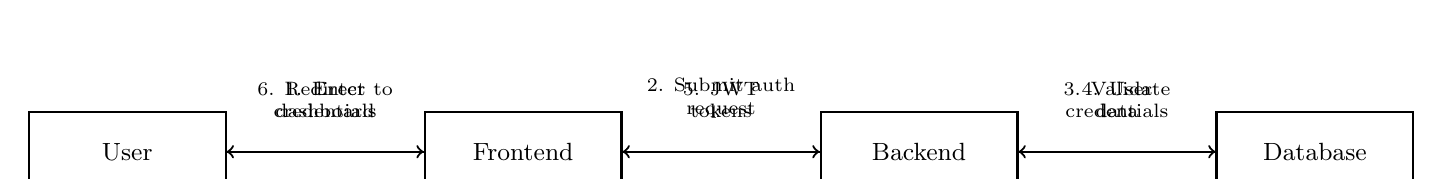
\begin{tikzpicture}[thick, node distance=2.5cm, every node/.style={align=center, font=\small}]
        \node (user) [draw, rectangle, minimum width=2.5cm, minimum height=1cm] {User};
        \node (frontend) [draw, rectangle, minimum width=2.5cm, minimum height=1cm, right=of user] {Frontend};
        \node (backend) [draw, rectangle, minimum width=2.5cm, minimum height=1cm, right=of frontend] {Backend};
        \node (database) [draw, rectangle, minimum width=2.5cm, minimum height=1cm, right=of backend] {Database};
        
        \draw[->] (user) -- (frontend) node[midway, above, font=\scriptsize, yshift=0.3cm] {1. Enter\\credentials};
        \draw[->] (frontend) -- (backend) node[midway, above, font=\scriptsize, yshift=0.3cm] {2. Submit auth\\request};
        \draw[->] (backend) -- (database) node[midway, above, font=\scriptsize, yshift=0.3cm] {3. Validate\\credentials};
        \draw[->] (database) -- (backend) node[midway, above, font=\scriptsize, yshift=0.3cm] {4. User\\data};
        \draw[->] (backend) -- (frontend) node[midway, above, font=\scriptsize, yshift=0.3cm] {5. JWT\\tokens};
        \draw[->] (frontend) -- (user) node[midway, above, font=\scriptsize, yshift=0.3cm] {6. Redirect to\\dashboard};
    \end{tikzpicture}
    \caption{Authentication Flow}
    \label{fig:auth-flow}
\end{figure}

\subsection{Token Management}

\begin{itemize}
    \item Access tokens with 15-minute expiry for security
    \item Refresh tokens with 7-day expiry for convenience
    \item Automatic token refresh before expiry
    \item Secure storage of tokens in HTTP-only cookies
\end{itemize}

\section{Assignment Management Workflow}

The assignment management system facilitates the creation, distribution, and evaluation of academic assignments.

\subsection{Assignment Creation Process}

\begin{enumerate}
    \item Teacher navigates to assignment creation interface
    \item Teacher fills in assignment details (title, description, due date, etc.)
    \item Teacher attaches any necessary files or resources
    \item Teacher selects target course and students
    \item Assignment is saved to the database
    \item Notifications are sent to relevant students
    \item Assignment appears in students' assignment lists
\end{enumerate}

\subsection{Assignment Submission Process}

\begin{enumerate}
    \item Student views assignment in their assignment list
    \item Student prepares submission (writes response, attaches files)
    \item Student submits assignment through the platform
    \item Submission is stored in the database
    \item Teacher receives notification of new submission
    \item Submission appears in teacher's evaluation queue
\end{enumerate}

\begin{figure}[H]
    \centering
    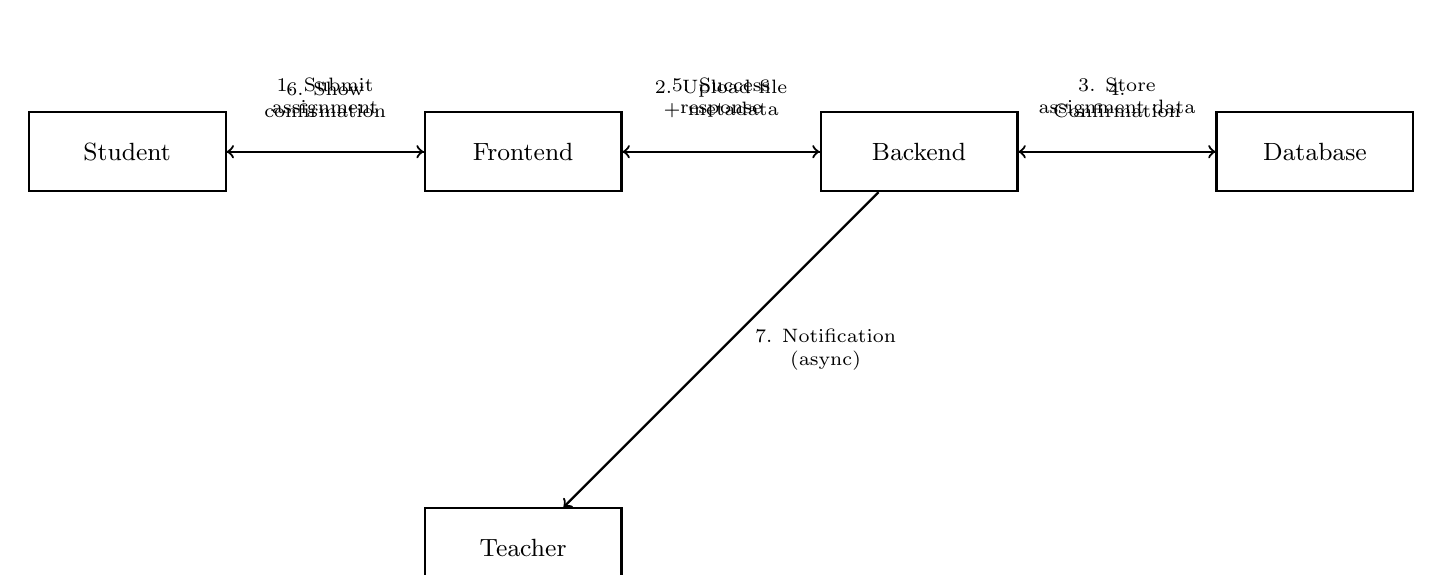
\begin{tikzpicture}[thick, node distance=2.5cm, every node/.style={align=center, font=\small}]
        \node (student) [draw, rectangle, minimum width=2.5cm, minimum height=1cm] {Student};
        \node (frontend) [draw, rectangle, minimum width=2.5cm, minimum height=1cm, right=of student] {Frontend};
        \node (backend) [draw, rectangle, minimum width=2.5cm, minimum height=1cm, right=of frontend] {Backend};
        \node (database) [draw, rectangle, minimum width=2.5cm, minimum height=1cm, right=of backend] {Database};
        \node (teacher) [draw, rectangle, minimum width=2.5cm, minimum height=1cm, below=of frontend, yshift=-1.5cm] {Teacher};
        
        \draw[->] (student) -- (frontend) node[midway, above, font=\scriptsize, yshift=0.3cm] {1. Submit\\assignment};
        \draw[->] (frontend) -- (backend) node[midway, above, font=\scriptsize, yshift=0.3cm] {2. Upload file\\+ metadata};
        \draw[->] (backend) -- (database) node[midway, above, font=\scriptsize, yshift=0.3cm] {3. Store\\assignment data};
        \draw[->] (database) -- (backend) node[midway, above, font=\scriptsize, yshift=0.3cm] {4.\\Confirmation};
        \draw[->] (backend) -- (frontend) node[midway, above, font=\scriptsize, yshift=0.3cm] {5. Success\\response};
        \draw[->] (frontend) -- (student) node[midway, above, font=\scriptsize, yshift=0.3cm] {6. Show\\confirmation};
        \draw[->] (backend) -- (teacher) node[midway, right, font=\scriptsize, xshift=0.3cm] {7. Notification\\(async)};
    \end{tikzpicture}
    \caption{Assignment Submission Flow}
    \label{fig:assignment-flow}
\end{figure}

\section{Grade Management Workflow}

The grade management system provides teachers with tools to evaluate student performance and students with access to their academic progress.

\subsection{Grade Entry Process}

\begin{enumerate}
    \item Teacher accesses grade entry interface
    \item Teacher selects course and assignment/exam
    \item Teacher enters grades for individual students
    \item System validates grade format and range
    \item Grades are saved to the database
    \item Grade calculations are updated (averages, totals)
    \item Students receive notifications of grade updates
\end{enumerate}

\subsection{Grade Viewing Process}

\begin{enumerate}
    \item Student navigates to grade viewing section
    \item System retrieves student's grades from database
    \item Grades are organized by course and term
    \item Visual representations (charts, graphs) are generated
    \item Student views grades and performance metrics
\end{enumerate}

\section{Attendance Tracking Workflow}

The attendance system helps track student participation and engagement in classes.

\subsection{Attendance Recording Process}

\begin{enumerate}
    \item Teacher opens attendance interface for a specific class
    \item System displays enrolled students for that class
    \item Teacher marks attendance status for each student
    \item Attendance data is saved to the database
    \item Attendance statistics are updated
    \item Notifications may be sent for attendance concerns
\end{enumerate}

\subsection{Attendance Viewing Process}

\begin{enumerate}
    \item Student or admin accesses attendance records
    \item System retrieves attendance data from database
    \item Data is organized by course and date
    \item Attendance percentages and trends are calculated
    \item Visual reports are generated
\end{enumerate}

\section{Billing and Payment Workflow}

The financial management system handles tuition, fees, and other monetary transactions.

\subsection{Billing Process}

\begin{enumerate}
    \item Admin creates billing records for students
    \item System calculates amounts based on course enrollment
    \item Billing records are stored in the database
    \item Invoices are generated and sent to students
    \item Payment due dates are tracked
\end{enumerate}

\subsection{Payment Process}

\begin{enumerate}
    \item Student accesses billing and payment interface
    \item Student views outstanding bills and due dates
    \item Student selects payment method and amount
    \item Payment information is processed securely
    \item Payment confirmation is recorded in the database
    \item Receipts are generated and sent to student
\end{enumerate}

\section{Communication Workflow}

The communication system facilitates announcements, notifications, and messaging between users.

\subsection{Announcement Creation Process}

\begin{enumerate}
    \item Admin or teacher creates an announcement
    \item Announcement details are entered (title, content, audience)
    \item Target audience is selected (all users, specific roles, etc.)
    \item Announcement is saved to the database
    \item Notifications are sent to target audience
    \item Announcement appears in relevant users' feeds
\end{enumerate}

\subsection{Notification Delivery Process}

\begin{enumerate}
    \item System event triggers a notification
    \item Notification is created and stored in database
    \item Notification is formatted for delivery
    \item Notification is sent via preferred channels (in-app, email, SMS)
    \item User receives notification
    \item User interaction with notification is tracked
\end{enumerate}

\section{Data Synchronization}

Campus-Sync implements real-time data synchronization to ensure all users have access to the most current information.

\subsection{Real-Time Updates}

\begin{itemize}
    \item WebSocket connections for live data updates
    \item Database triggers for immediate change notifications
    \item Client-side caching for improved performance
    \item Conflict resolution for concurrent updates
\end{itemize}

\subsection{Offline Support}

\begin{itemize}
    \item Local data storage for offline access
    \item Synchronization queue for offline actions
    \item Conflict detection and resolution
    \item Automatic sync when connectivity is restored
\end{itemize}

\section{Error Handling and Recovery}

The system implements comprehensive error handling to ensure reliability and user experience.

\subsection{Error Types}

\begin{itemize}
    \item Validation errors (input format issues)
    \item Authentication errors (login failures)
    \item Authorization errors (access denied)
    \item Database errors (connection failures, query issues)
    \item Server errors (500-level HTTP errors)
    \item Network errors (connectivity issues)
\end{itemize}

\subsection{Error Response Format}

\begin{lstlisting}[language=JSON, caption=Error Response Format]
{
  "success": false,
  "error": {
    "code": "VALIDATION_ERROR",
    "message": "Validation failed",
    "details": [
      {
        "field": "email",
        "message": "Email is required"
      }
    ]
  }
}
\end{lstlisting}

\subsection{Recovery Mechanisms}

\begin{itemize}
    \item Automatic retry for transient failures
    \item Graceful degradation for non-critical features
    \item User-friendly error messages
    \item Logging for debugging and monitoring
\end{itemize}

This workflow documentation provides a comprehensive overview of how data flows through the Campus-Sync platform and how various processes are executed, ensuring a clear understanding of system operations for developers, administrators, and stakeholders.
\chapter{Future Implementations and Roadmap}

\section{Strategic Vision}

Campus-Sync is designed as a living platform that will continue to evolve and expand to meet the changing needs of educational institutions. The future development roadmap focuses on enhancing automation, improving communication, and integrating with external services to create a more intelligent and efficient educational ecosystem.

\section{n8n Workflow Automation Integration}

One of the key future enhancements for Campus-Sync is the integration of n8n, a powerful workflow automation engine that will orchestrate complex business processes and connect the platform with external services.

\subsection{Integration Overview}

n8n will serve as the core workflow automation engine, streamlining institutional operations and enhancing user experience through intelligent automation across all panel types. This integration will significantly reduce manual overhead while improving user engagement and institutional efficiency.

\subsection{Panel-Specific Automation Workflows}

\subsubsection{Administrative Panel Automation}

\begin{itemize}
    \item \textbf{User Management}: Automated provisioning and deprovisioning of student/teacher accounts
    \item \textbf{Course Planning}: Intelligent academic calendar generation and course scheduling
    \item \textbf{Billing Workflows}: End-to-end automation of invoice generation and distribution
    \item \textbf{Report Generation}: Automated production of institutional analytics and compliance reports
    \item \textbf{System Maintenance}: Scheduled backups, updates, and performance optimization
\end{itemize}

\subsubsection{Teacher Panel Automation}

\begin{itemize}
    \item \textbf{Assignment Distribution}: Automated assignment creation and distribution to students
    \item \textbf{Grade Publishing}: Automated dissemination of grade reports upon publication
    \item \textbf{Attendance Processing}: Automated attendance roll call and reporting
    \item \textbf{Class Communication}: Scheduled class announcements and resource distribution
    \item \textbf{Performance Analytics}: Automated generation of student performance insights
\end{itemize}

\subsubsection{Student Panel Automation}

\begin{itemize}
    \item \textbf{Academic Notifications}: Proactive engagement for assignments, exams, and grades
    \item \textbf{Study Reminders}: Personalized academic scheduling based on learning patterns
    \item \textbf{Resource Recommendations}: AI-driven content and activity suggestions
    \item \textbf{Progress Tracking}: Automated academic progress reporting and alerts
    \item \textbf{Wellness Integration}: Stress-adaptive wellness session planning
\end{itemize}

\begin{figure}[H]
    \centering
    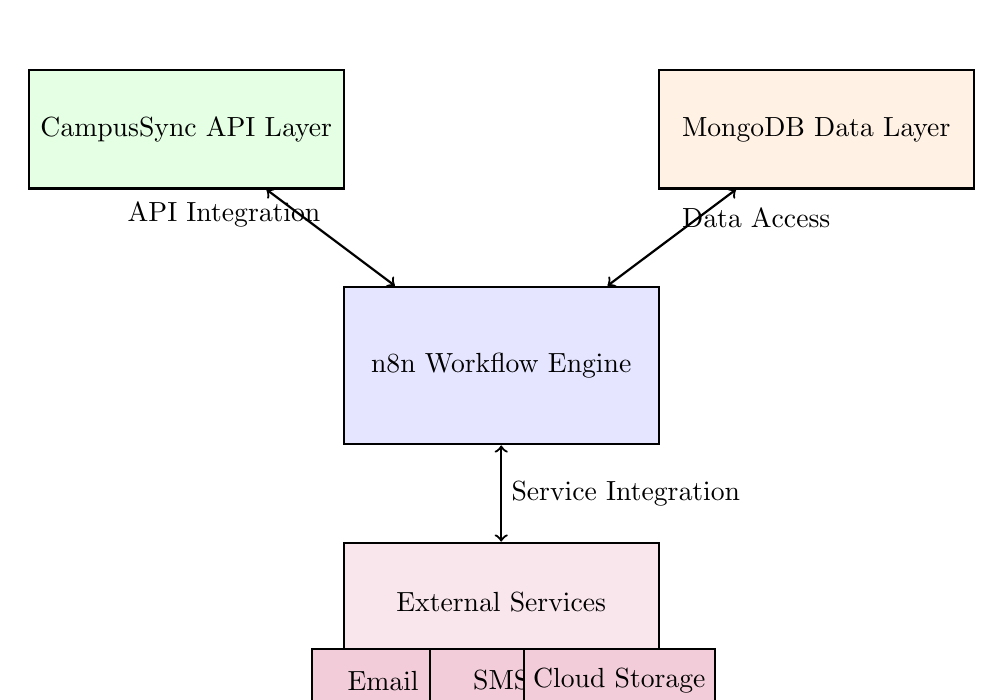
\begin{tikzpicture}[thick]
        % n8n Workflow Engine
        \node[draw, rectangle, minimum width=4cm, minimum height=2cm, fill=blue!10] (n8n) at (0,0) {n8n Workflow Engine};
        
        % CampusSync API
        \node[draw, rectangle, minimum width=4cm, minimum height=1.5cm, fill=green!10] (api) at (-4,3) {CampusSync API Layer};
        
        % Database
        \node[draw, rectangle, minimum width=4cm, minimum height=1.5cm, fill=orange!10] (database) at (4,3) {MongoDB Data Layer};
        
        % External Services
        \node[draw, rectangle, minimum width=4cm, minimum height=1.5cm, fill=purple!10] (external) at (0,-3) {External Services};
        \node[draw, rectangle, minimum width=1.8cm, minimum height=0.8cm, fill=purple!20] (email) at (-1.5,-4) {Email};
        \node[draw, rectangle, minimum width=1.8cm, minimum height=0.8cm, fill=purple!20] (sms) at (0,-4) {SMS};
        \node[draw, rectangle, minimum width=1.8cm, minimum height=0.8cm, fill=purple!20] (cloud) at (1.5,-4) {Cloud Storage};
        
        % Arrows
        \draw[<->] (api) -- (n8n) node[midway, above left] {API Integration};
        \draw[<->] (database) -- (n8n) node[midway, above right] {Data Access};
        \draw[<->] (n8n) -- (external) node[midway, right] {Service Integration};
    \end{tikzpicture}
    \caption{n8n Integration Architecture}
    \label{fig:n8n-integration}
\end{figure}

\section{Enterprise Communication Integration}

\subsection{Email Integration}

The platform will integrate with enterprise email services to provide robust communication capabilities:

\subsubsection{Service Providers}

\begin{itemize}
    \item \textbf{Primary}: SendGrid (High deliverability, advanced analytics)
    \item \textbf{Secondary}: Amazon SES (Cost-effective, scalable)
    \item \textbf{Tertiary}: Mailgun (Redundancy, global delivery)
\end{itemize}

\subsubsection{Advanced Email Features}

\begin{itemize}
    \item \textbf{Dynamic Template Engine}: Role-specific content personalization
    \item \textbf{Behavioral Triggering}: Event-based communication workflows
    \item \textbf{Delivery Scheduling}: Time-zone aware message optimization
    \item \textbf{Comprehensive Analytics}: Real-time engagement metrics and A/B testing
    \item \textbf{Compliance Management}: GDPR/FERPA compliant communication protocols
\end{itemize}

\subsection{SMS Integration}

Global SMS integration will provide instant communication capabilities:

\subsubsection{Service Provider Ecosystem}

\begin{itemize}
    \item \textbf{Global Coverage}: Twilio (99.9\% uptime, extensive network)
    \item \textbf{Regional Optimization}: Vonage (Cost-effective local routing)
    \item \textbf{Emergency Redundancy}: Plivo (Backup communication channel)
\end{itemize}

\subsubsection{Enterprise SMS Capabilities}

\begin{itemize}
    \item \textbf{Priority Queuing}: Mission-critical message prioritization
    \item \textbf{Multi-Factor Authentication}: Secure access verification protocols
    \item \textbf{Emergency Broadcasting}: Instant mass-notification system
    \item \textbf{Delivery Scheduling}: Time-zone optimized message delivery
    \item \textbf{Cost Optimization}: Intelligent routing for economical delivery
\end{itemize}

\section{External Service Integration}

Campus-Sync will integrate with various external services to extend its capabilities and provide a more comprehensive educational environment.

\subsection{Learning Management Ecosystem}

\begin{itemize}
    \item \textbf{Google Classroom}: Seamless content and assignment synchronization
    \item \textbf{Microsoft Teams}: Native integration with Office 365 environments
    \item \textbf{Canvas/Moodle}: Bidirectional data exchange and interoperability
\end{itemize}

\subsection{Productivity Platform Integration}

\begin{itemize}
    \item \textbf{Google Workspace}: Calendar, Drive, and Docs synchronization
    \item \textbf{Microsoft 365}: Teams, Outlook, and SharePoint connectivity
    \item \textbf{Slack/Discord}: Community engagement and collaboration channels
\end{itemize}

\subsection{Financial Services Integration}

\begin{itemize}
    \item \textbf{Stripe/PayPal}: Multi-channel payment processing
    \item \textbf{Regional Payment Gateways}: Local payment method support
    \item \textbf{Accounting Systems}: QuickBooks, Xero integration for financial reporting
\end{itemize}

\subsection{Cloud Storage Federation}

\begin{itemize}
    \item \textbf{Google Drive}: Document management and sharing
    \item \textbf{Dropbox}: Enterprise file synchronization
    \item \textbf{OneDrive}: Microsoft ecosystem integration
    \item \textbf{Box}: Enterprise-grade content management
\end{itemize}

\section{Advanced Automation Scenarios}

\subsection{Intelligence Workflows}

\begin{itemize}
    \item \textbf{Administrative Risk Assessment}: Machine learning-based institutional efficiency prediction
    \item \textbf{Teacher Adaptive Learning Paths}: Dynamic curriculum adjustment algorithms
    \item \textbf{Student Resource Allocation}: Demand forecasting and optimization
    \item \textbf{Cross-Panel Personalized Recommendations}: AI-driven content and activity suggestions
\end{itemize}

\subsection{Context-Aware Communication}

\begin{itemize}
    \item \textbf{Location-Based Notifications}: Geo-fencing for campus services
    \item \textbf{Behavioral Pattern Recognition}: Usage-based engagement optimization
    \item \textbf{Collaborative Workflows}: Cross-panel project coordination
    \item \textbf{Feedback-Driven Improvement}: Continuous system optimization
\end{itemize}

\section{Enterprise Security and Compliance}

Future implementations will enhance security and compliance capabilities to meet enterprise standards.

\subsection{Data Protection Protocols}

\begin{itemize}
    \item \textbf{End-to-End Encryption}: AES-256 communication security
    \item \textbf{Role-Based Access Control}: Granular permission management by panel
    \item \textbf{Comprehensive Audit Trails}: Complete action logging and tracking
    \item \textbf{Regulatory Compliance}: GDPR, FERPA, HIPAA alignment
\end{itemize}

\subsection{Authentication Security}

\begin{itemize}
    \item \textbf{OAuth 2.0 Integration}: Secure third-party service authentication
    \item \textbf{API Key Management}: Rotating credential security protocols
    \item \textbf{Rate Limiting}: Abuse prevention and system protection
    \item \textbf{Real-Time Monitoring}: Anomaly detection and threat response
\end{itemize}

\section{Implementation Roadmap}

The future development of Campus-Sync follows a phased approach to ensure smooth integration and minimal disruption to existing operations.

\subsection{Phase 1: Foundation (Months 1-2)}

\begin{itemize}
    \item n8n infrastructure provisioning and configuration
    \item Core email and SMS service integration
    \item Basic notification workflow deployment
    \item Monitoring and analytics framework establishment
\end{itemize}

\subsection{Phase 2: Administrative Enhancement (Months 3-4)}

\begin{itemize}
    \item Comprehensive administrative workflow automation
    \item User management and course planning automation
    \item Report generation and analytics implementation
    \item Delivery optimization and performance tuning
\end{itemize}

\subsection{Phase 3: Teacher Integration (Months 5-6)}

\begin{itemize}
    \item Teacher workflow automation deployment
    \item Assignment and grade processing automation
    \item Class communication and analytics implementation
    \item Enhanced security protocol deployment
\end{itemize}

\subsection{Phase 4: Student Optimization (Months 7-8)}

\begin{itemize}
    \item Student engagement automation systems
    \item Academic progress tracking and alerts
    \item Wellness and productivity integration
    \item User experience optimization initiatives
\end{itemize}

\subsection{Phase 5: Cross-Panel Integration (Months 9-12)}

\begin{itemize}
    \item Cross-panel workflow orchestration
    \item AI-powered automation workflows
    \item Productivity platform integration
    \item Comprehensive monitoring dashboard launch
\end{itemize}

\section{Investment Analysis}

\subsection{Operational Expenditure}

\begin{itemize}
    \item \textbf{n8n Hosting}: \$50-200/month (scalable infrastructure)
    \item \textbf{Communication Services}: \$100-300/month (email/SMS volume-based)
    \item \textbf{API Integration}: \$50-150/month (third-party service fees)
    \item \textbf{Monitoring Tools}: \$50-100/month (analytics and observability)
\end{itemize}

\subsection{Resource Investment}

\begin{itemize}
    \item \textbf{Infrastructure}: Dedicated automation server resources
    \item \textbf{Development}: Specialized workflow engineering personnel
    \item \textbf{Operations}: System monitoring and maintenance staff
    \item \textbf{Support}: User assistance for automated features
\end{itemize}

\section{Key Performance Indicators}

\subsection{Quantitative Metrics}

\begin{itemize}
    \item \textbf{Operational Efficiency}: Hours saved through process automation
    \item \textbf{User Engagement}: Platform usage increase and retention rates
    \item \textbf{Communication Effectiveness}: Improved delivery and response metrics
    \item \textbf{Error Reduction}: Decreased manual intervention requirements
\end{itemize}

\subsection{Qualitative Assessments}

\begin{itemize}
    \item \textbf{User Satisfaction}: Stakeholder feedback and satisfaction scores
    \item \textbf{Administrative Productivity}: Staff efficiency and workflow improvements
    \item \textbf{Academic Outcomes}: Measurable impact on student performance
    \item \textbf{System Reliability}: Uptime, performance, and scalability metrics
\end{itemize}

\section{Emerging Technology Integration}

\subsection{Future Expansion Opportunities}

\begin{itemize}
    \item \textbf{Machine Learning}: Advanced predictive analytics and automation
    \item \textbf{Internet of Things}: Smart campus device and sensor integration
    \item \textbf{Blockchain}: Immutable academic credential verification
    \item \textbf{Immersive Technologies}: AR/VR-enhanced learning experiences
\end{itemize}

\subsection{Market Development}

\begin{itemize}
    \item \textbf{Corporate Education}: Enterprise training platform adaptation
    \item \textbf{Primary/Secondary Education}: K-12 optimized feature sets
    \item \textbf{Higher Education}: Research-focused advanced capabilities
    \item \textbf{Global Markets}: Localization and international compliance
\end{itemize}

\section{Conclusion}

The future development roadmap for Campus-Sync positions the platform as a next-generation educational solution. By leveraging cutting-edge automation technologies, enterprise-grade communication systems, and strategic external service integrations, Campus-Sync will continue to evolve into an intelligent, efficient, and engaging learning environment.

The integration of n8n workflow automation, comprehensive communication systems, and advanced security measures will establish Campus-Sync as a leader in educational technology innovation. This strategic enhancement roadmap ensures that the platform remains at the forefront of educational technology while meeting the evolving needs of students, teachers, and administrators in the digital age.

% Bibliography
\newpage
\begin{thebibliography}{9}
\bibitem{react}
React Documentation. \url{https://reactjs.org/docs/getting-started.html}
\bibitem{vite}
Vite Documentation. \url{https://vitejs.dev/guide/}
\bibitem{supabase}
Supabase Documentation. \url{https://supabase.com/docs}
\bibitem{tailwind}
Tailwind CSS Documentation. \url{https://tailwindcss.com/docs}
\bibitem{shadcn}
shadcn/ui Documentation. \url{https://ui.shadcn.com/docs}
\bibitem{typescript}
TypeScript Documentation. \url{https://www.typescriptlang.org/docs/}
\end{thebibliography}

\end{document}